
\begin{table}
  \centering
  \begin{tabular}{@{}rrrrrr@{}}
    {}    & \multicolumn{1}{c}{$b$} & \multicolumn{1}{c}{$c$} & \multicolumn{1}{c}{$uds$} & \multicolumn{1}{c}{$g$} & non-$q$-matched     \\ 
    \midrule
    2 & \SI{37.2}{\percent}  & \SI{12.9}{\percent}  & \SI{29.1}{\percent} &  \SI{0.0}{\percent} & \SI{20.7}{\percent}  \\
    3 & \SI{22.6}{\percent}  &  \SI{8.9}{\percent}  & \SI{19.7}{\percent} & \SI{31.2}{\percent} & \SI{17.5}{\percent}  \\
    4 & \SI{14.6}{\percent}  &  \SI{7.0}{\percent}  & \SI{15.0}{\percent} & \SI{45.1}{\percent} & \SI{18.3}{\percent}  \\
    5 & \SI{10.0}{\percent}  &  \SI{5.7}{\percent}  & \SI{12.2}{\percent} & \SI{52.5}{\percent} & \SI{19.6}{\percent}  \\
    6 &  \SI{7.1}{\percent}  &  \SI{4.4}{\percent}  &  \SI{8.8}{\percent} & \SI{54.4}{\percent} & \SI{25.2}{\percent}  \\
  \end{tabular}
  \caption{Number of different types of jets for MC and MCb written in relative numbers such that each row sum to \SI{100}{\percent}. See also Table~\ref{tab:q:flevt_overview}.}
  \label{tab:q:flevt_overview_percent_relative}
\end{table}


\newpage
\begin{figure*}[h!]
  \centerfloat
  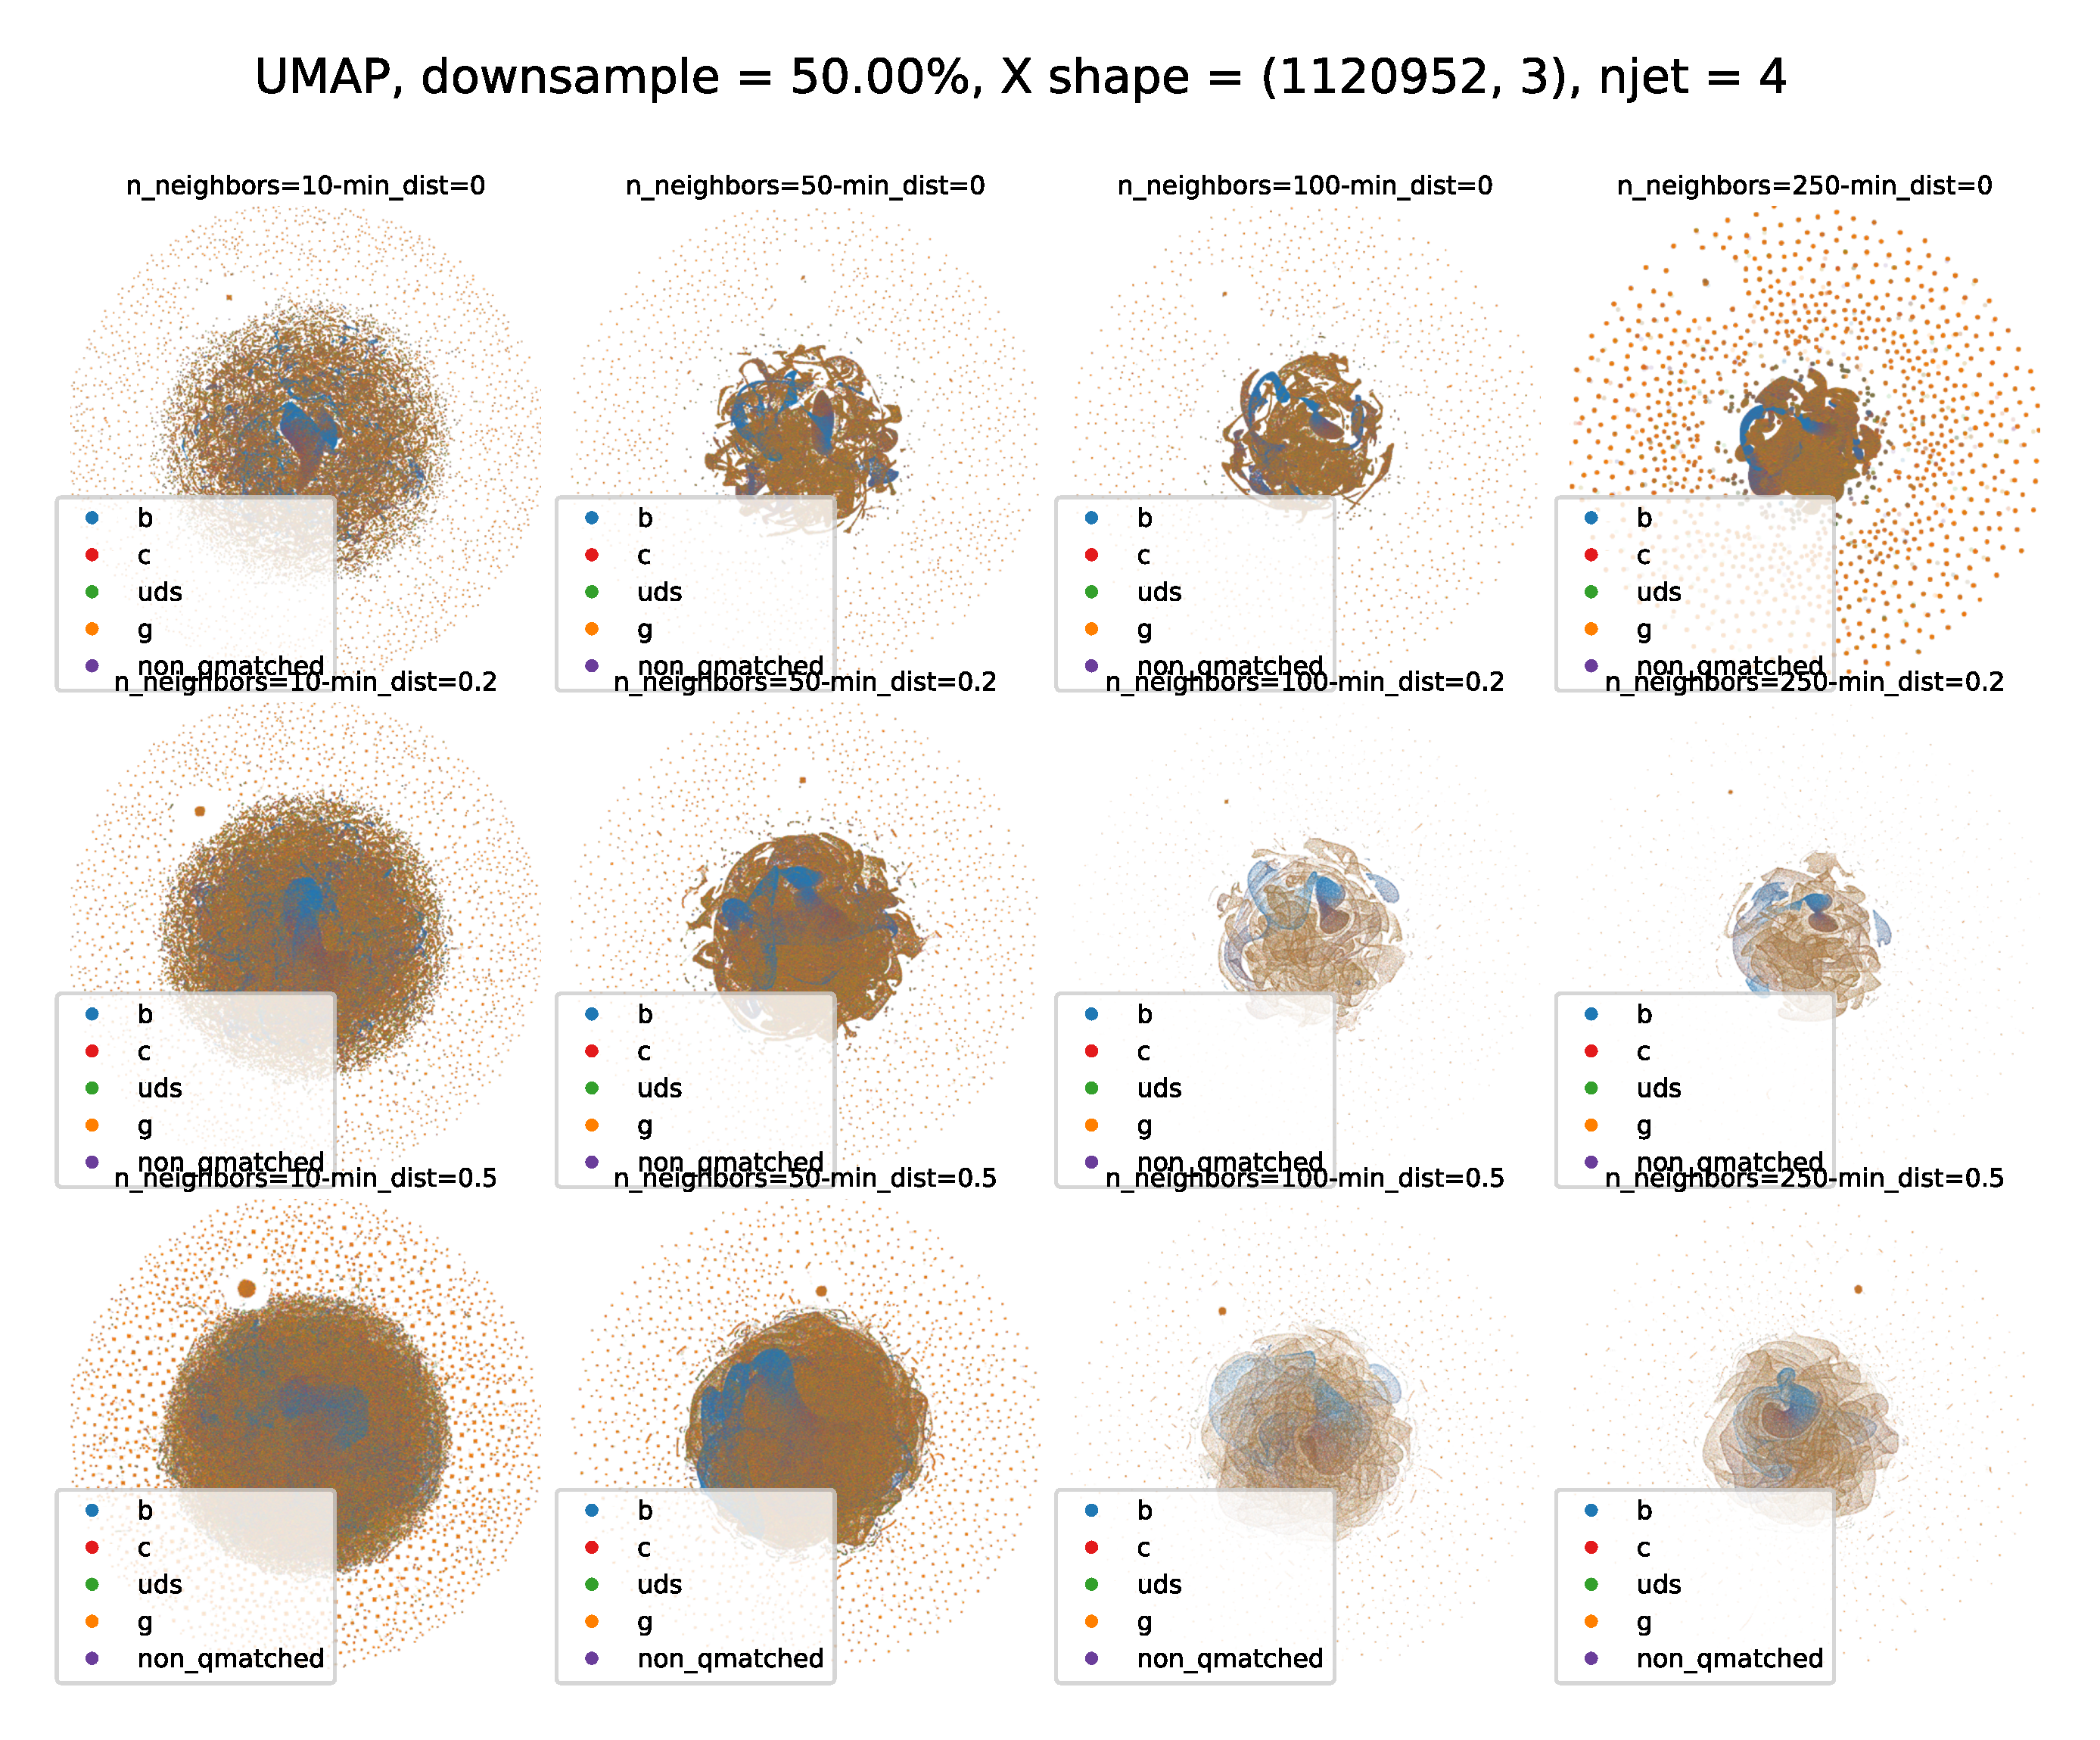
\includegraphics[draft=false, width=0.98\textwidth, trim=30 30 30 70, clip]{figures/quarks/viz_UMAP_test_0.5_input2b_njet=4_algorithm=UMAP.pdf}
  \caption[UMAP Parameter Grid Search]
          {Grid search of the two parameters \code{n_neighbors} and \code{min_dist} for the UMAP algorithm run on 4-jet events. For an explanation of these, see \autoref{sec:q:EDA}.} 
  \label{fig:q:UMAP_vertex_all_4j}
\end{figure*}

\vspace{2cm}

\begin{figure*}[h!]
  \centerfloat
  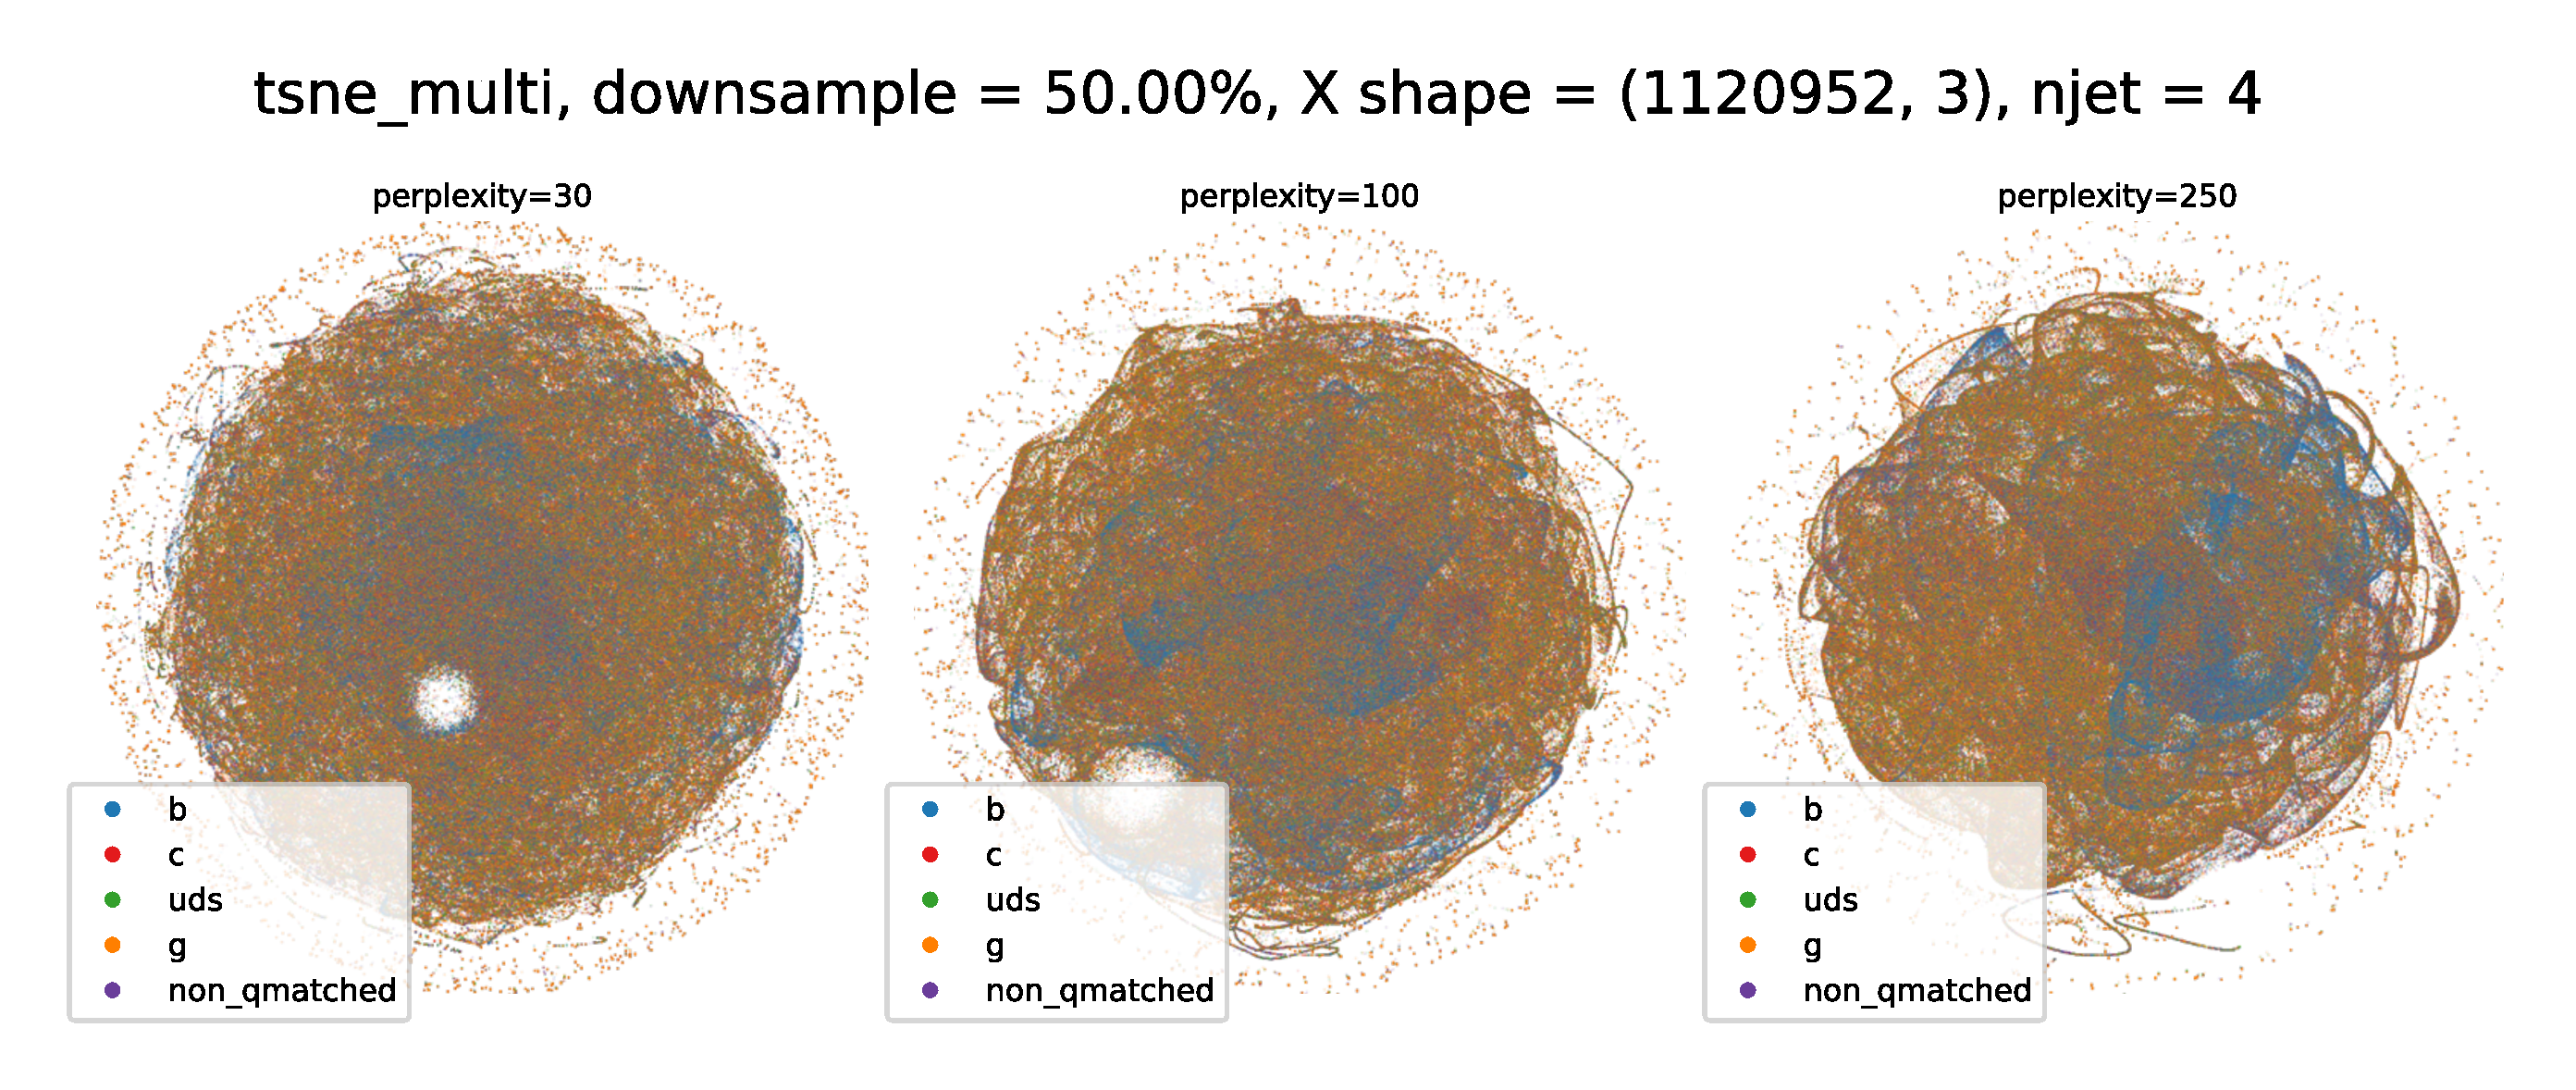
\includegraphics[draft=false, width=0.98\textwidth, trim=30 30 30 70, clip]{figures/quarks/viz_TSNE_MULTI_test_0.5_input2b_njet=4_algorithm=tsne_multi.pdf}
  \caption[Visualization of the t-SNE algorithm]
          {Visualization of the t-SNE algorithm as a function of the \code{perplexity} parameters for 4-jet events.} 
  \label{fig:q:tsne_vertex}
\end{figure*}

\FloatBarrier
\newpage


\begin{table}
  \centerfloat
  \begin{tabular}{@{}ll@{}}
  Hyperparameter                &  Range                                  \\ \midrule
  \code{subsample}              & $\mathcal{U}(0.4, 1)$                   \\
  \code{colsample_bytree}       & $\mathcal{U}_\mathrm{trunc}(0.4, 1, 2)$ \\
  \code{max_depth}              & $\mathcal{U}_\mathrm{int}(1, 20)$       \\
  \code{min_child_weight}       & $\mathcal{U}_\mathrm{int}(0, 10)$       \\
  \end{tabular}
  % \vspace{\abovecaptionskip}
  \vspace{3mm}
  \caption[Random Search PDFs for XGB]{\label{tab:q:hpo_ranges_xgb}Probability Density Functions for the random search hyperparameter optimization process for the XGBoost model.}
\end{table}


\begin{figure}
  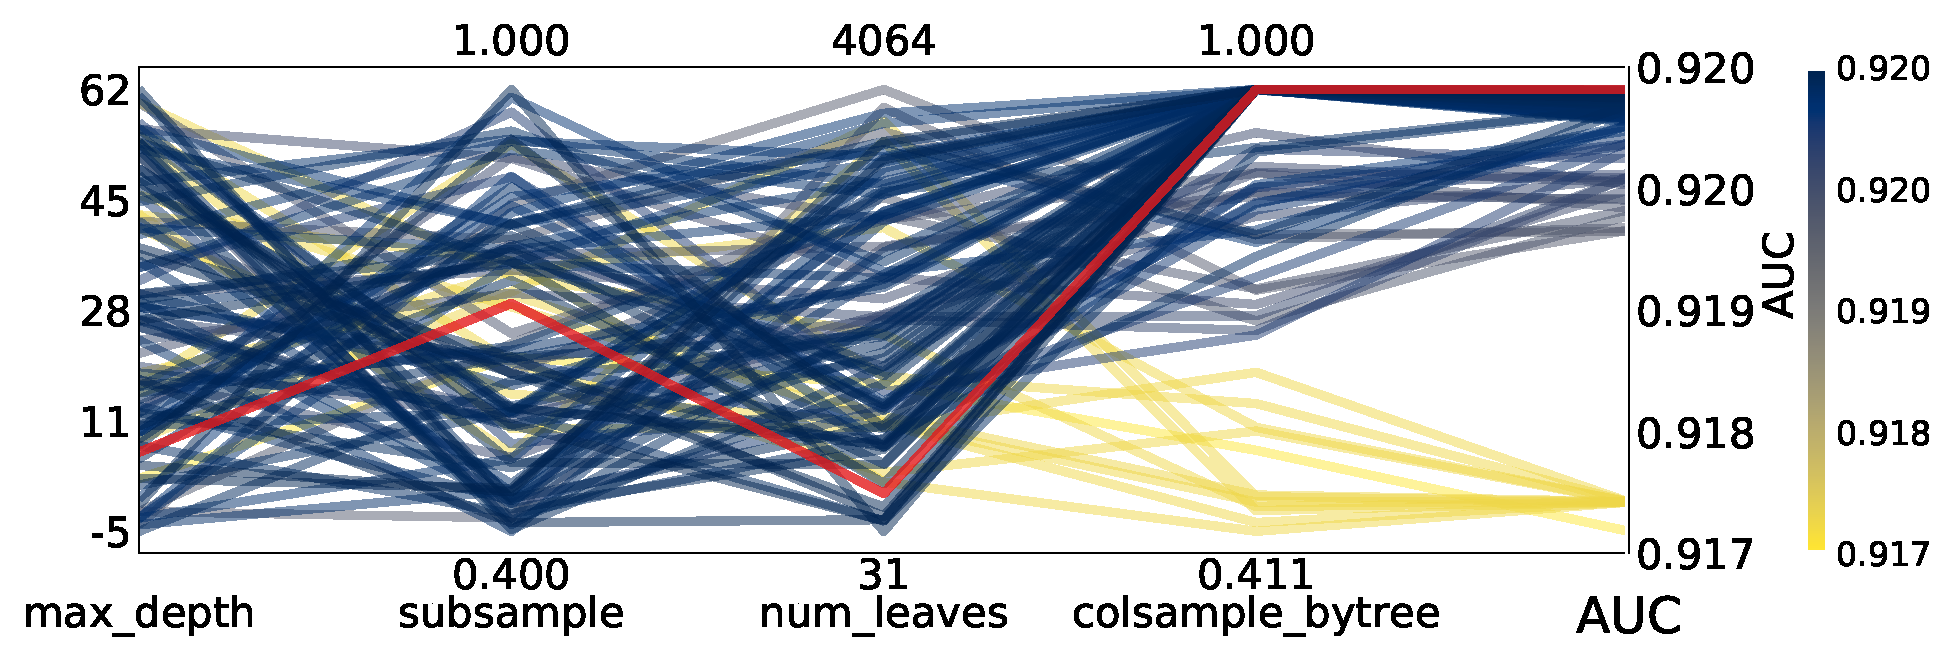
\includegraphics[width=0.98\textwidth, trim=0 0 0 0, clip]{figures/quarks/CV_viz-njet=3-name=lf_lgb_down_sample=1.00-ML_vars=vertex-selection=b-ejet_min=4-n_iter_RS_lgb=99-n_iter_RS_xgb=9-cdot_cut=0.90-version=19.pdf}
  \caption[Parallel Plot of HPO results for 3-jet $b$-Tagging]
          {Hyperparameter optimization results of $b$-tagging for 3-jet events. The results are shown as parallel coordinates with each hyperparameter along the $x$-axis and the value of that parameter on the $y$-axis. Each line is an event in the 4-dimensional space colored according to the performance of that hyperparameter as measured by AUC from \textcolor{viridis-dark}{highest} AUC in dark blue to \textcolor{viridis-light}{lowest} AUC in yellow. The \textcolor{red}{single best hyperparameter} is shown in red. 
          } 
  \label{fig:q:initial_CV_res_parallel_coords_3j}
\end{figure}


\begin{figure}
  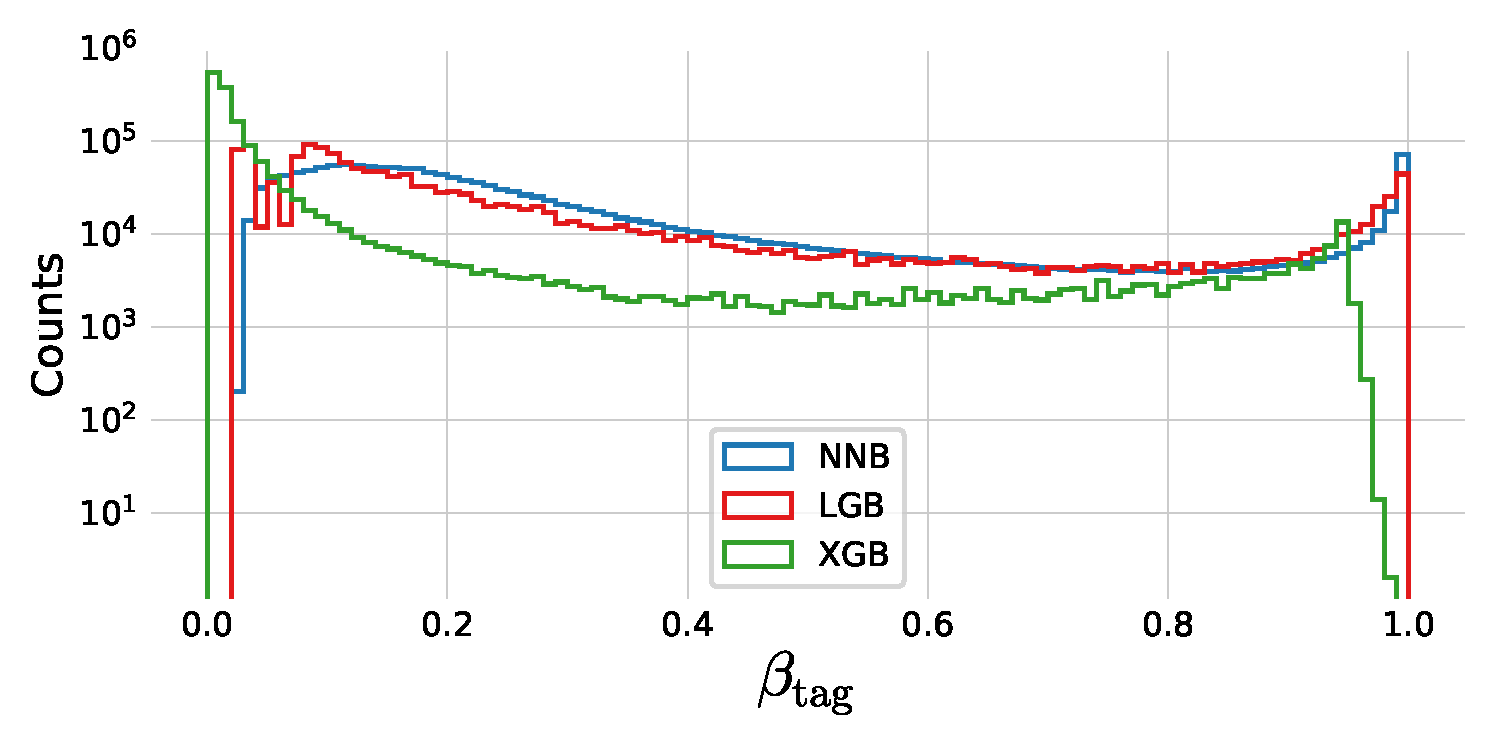
\includegraphics[width=0.95\textwidth, trim=0 0 0 30, clip]{figures/quarks/y_pred_3_jet_hist-down_sample=1.00-ML_vars=vertex-selection=b-ejet_min=4-n_iter_RS_lgb=99-n_iter_RS_xgb=9-cdot_cut=0.90-version=19.pdf}
  \caption[b-tag scores in 3-jet events]
          {Histogram of $b$-tag scores $\beta_\mathrm{tag}$ in 3-jet events for \textcolor{blue}{NNB} (the neural network pre-trained by ALEPH, also called \code{nnbjet}) in blue, \textcolor{red}{LGB} in red, and \textcolor{green}{XGB} in green. 
          } 
  \label{fig:q:btag_scores_3j}
\end{figure}


\begin{figure}
  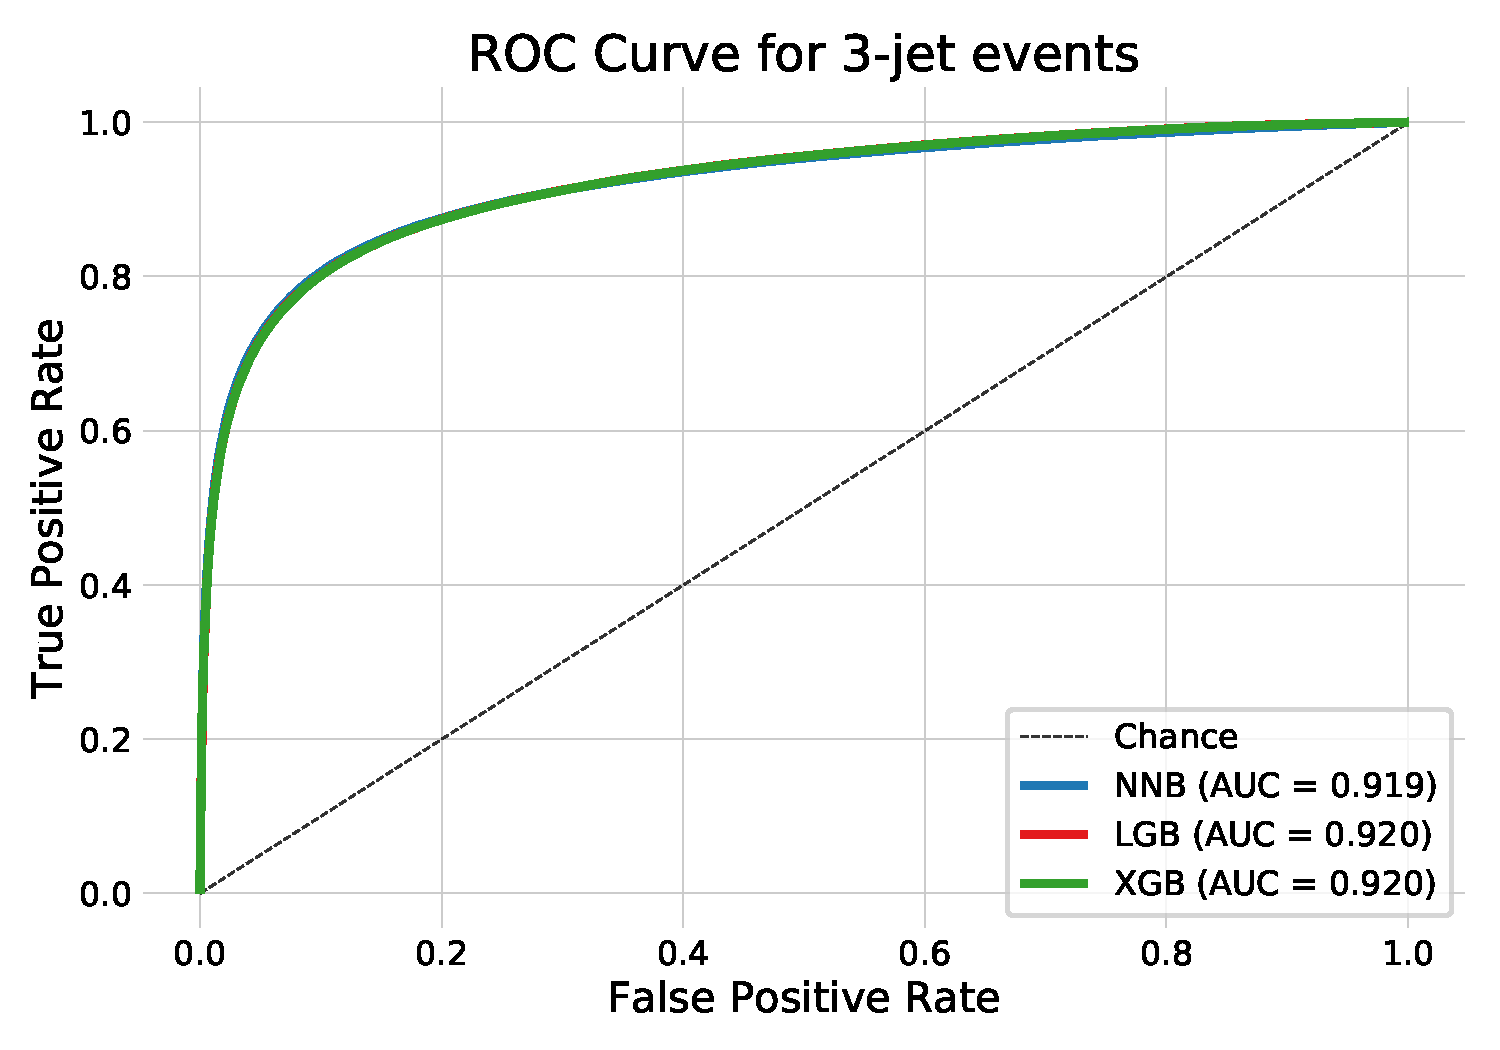
\includegraphics[width=0.95\textwidth, trim=10 10 10 40, clip]{figures/quarks/ROC_3_jet-down_sample=1.00-ML_vars=vertex-selection=b-ejet_min=4-n_iter_RS_lgb=99-n_iter_RS_xgb=9-cdot_cut=0.90-version=19.pdf}
  \caption[ROC curve for 3-jet $b$-tagging]
          {ROC curve of the three $b$-tag models in 3-jet events for \textcolor{blue}{NNB} (the pre-trained neural network trained by ALEPH, also called \code{nnbjet}) in blue, \textcolor{red}{LGB} in red, and \textcolor{green}{XGB} in green. In the legend the area under curve (AUC) is also shown. Notice that the LGB and XGB models share performance and it is thus due to overplotting that only the green line for XGB can be seen. In the machine learning community the background efficiency $\varepsilon_\mathrm{bkg}$ is sometimes know as the false positive rate (FPR) and the signal efficiency $\varepsilon_\mathrm{sig}$ as the true positive rate (TPR).  
          } 
  \label{fig:q:roc_btag_3j}
\end{figure}


\begin{figure}[h!]
    \centerfloat
    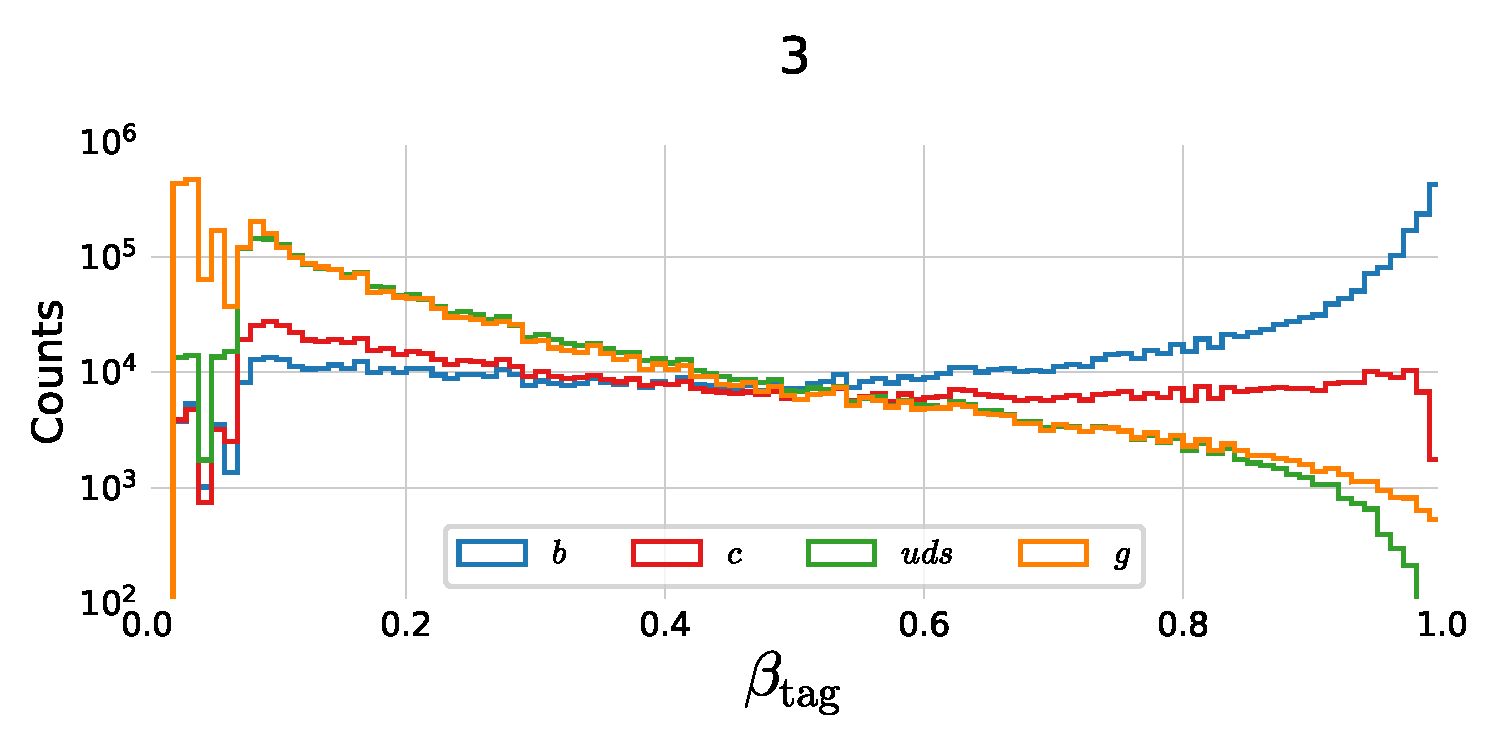
\includegraphics[width=0.95\textwidth, trim=15 15 15 50, clip]{figures/quarks/btag_scores_histogram_-njet=3-down_sample=1.00-ML_vars=vertex-selection=b-ejet_min=4-n_iter_RS_lgb=99-n_iter_RS_xgb=9-cdot_cut=0.90-version=19.pdf}
    \caption[Distribution of $b$-Tags in 3-Jet Events]
            {Distribution of $b$-tags in 3-jet events for \textcolor{blue}{$b$-jets} in blue, \textcolor{red}{$c$-jets} in red, \textcolor{green}{$uds$} in green and \textcolor{orange}{$g$} in orange.} 
    \label{fig:q:btag_histogram_3j}
  \end{figure}
  



\begin{figure}[h!]
  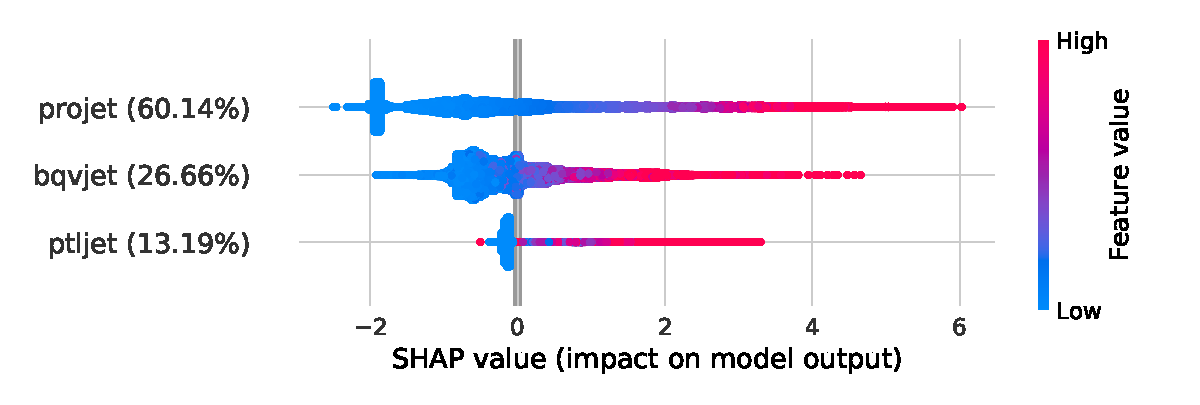
\includegraphics[width=0.98\textwidth, trim=10 10 20 10, clip]{figures/quarks/shap_global-down_sample=1.00-ML_vars=vertex-selection=b-ejet_min=4-n_iter_RS_lgb=99-n_iter_RS_xgb=9-cdot_cut=0.90-version=19-njet=3.pdf}
  \caption[Global Feature Importances for the LGB $b$-Tagging Algorithm on 3-Jet Events]
          {Global feature importances for the LGB $b$-tagging algorithm on 3-jet events. The normalized feature importance is shown in the parenthesis and the each dot is an observation showing the dependance between the SHAP value and the feature's value. 
          } 
  \label{fig:q:shap_btag_global_3j}
\end{figure}

\newpage
\FloatBarrier


\begin{figure}[h!]
  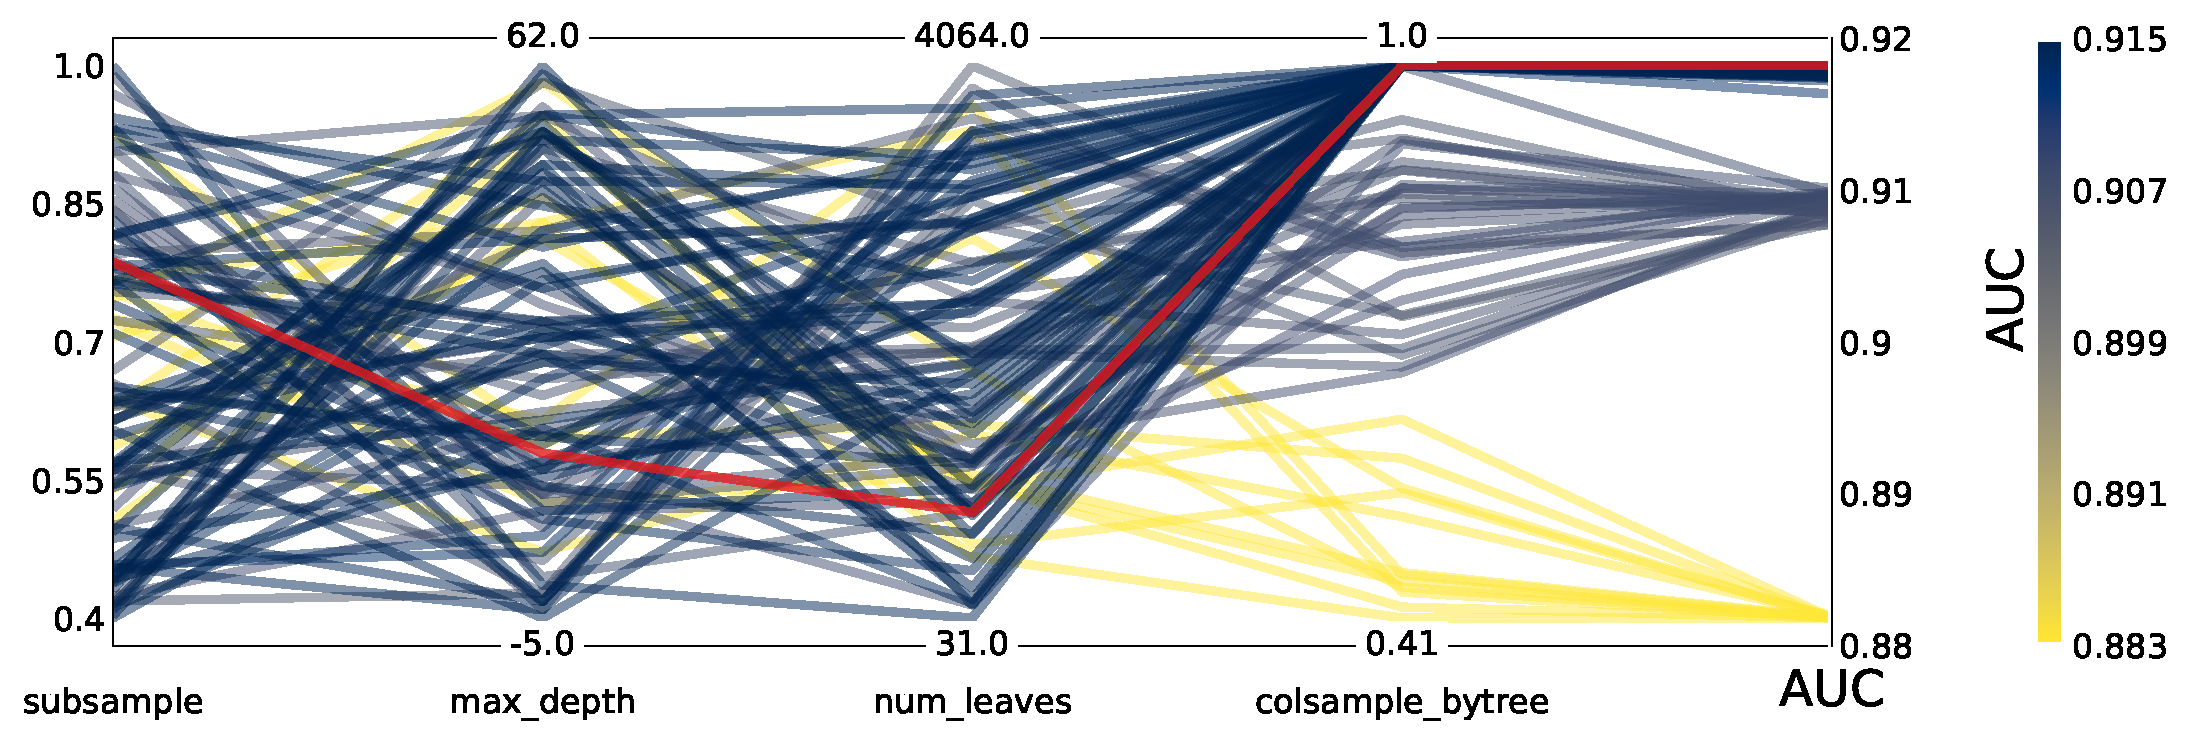
\includegraphics[width=0.98\textwidth, trim=0 0 0 0, clip]{figures/quarks/CV_viz-njet=3-name=lf_gtag_energy_ordered_lgb_down_sample=1.00-ML_vars=vertex-selection=b-ejet_min=4-n_iter_RS_lgb=99-n_iter_RS_xgb=9-cdot_cut=0.90-version=19.pdf}
  \caption[Parallel Plot of HPO Results for 3-Jet $g$-Tagging for Energy Ordered Jets]
          {Hyperparameter optimization results of $g$-tagging for 3-jet events for energy ordered jets. 
          } 
  \label{fig:q:CV_res_parallel_coords_g_tag_3j_energy_ordered}
\end{figure}


\begin{figure}[h!]
  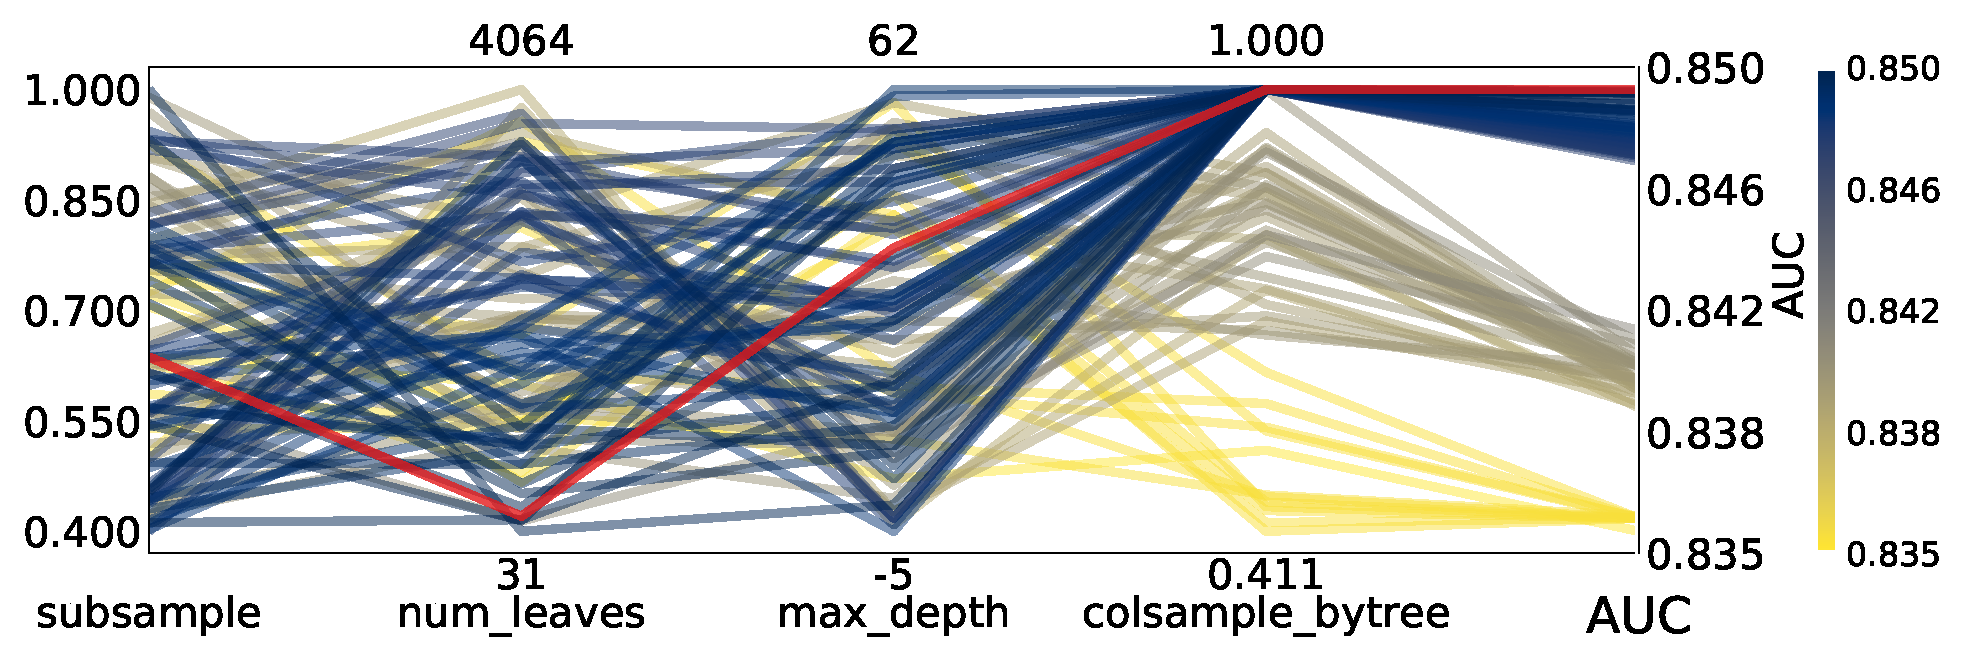
\includegraphics[width=0.98\textwidth, trim=0 0 0 0, clip]{figures/quarks/CV_viz-njet=3-name=lf_gtag_shuffled_lgb_down_sample=1.00-ML_vars=vertex-selection=b-ejet_min=4-n_iter_RS_lgb=99-n_iter_RS_xgb=9-cdot_cut=0.90-version=19.pdf}
  \caption[Parallel Plot of HPO Results for 3-Jet $g$-Tagging for Shuffled Jets]
          {Hyperparameter optimization results of $g$-tagging for 3-jet events for (row) shuffled jets. 
          } 
  \label{fig:q:CV_res_parallel_coords_g_tag_3j_shuffled}
\end{figure}

\begin{figure}[h!]
  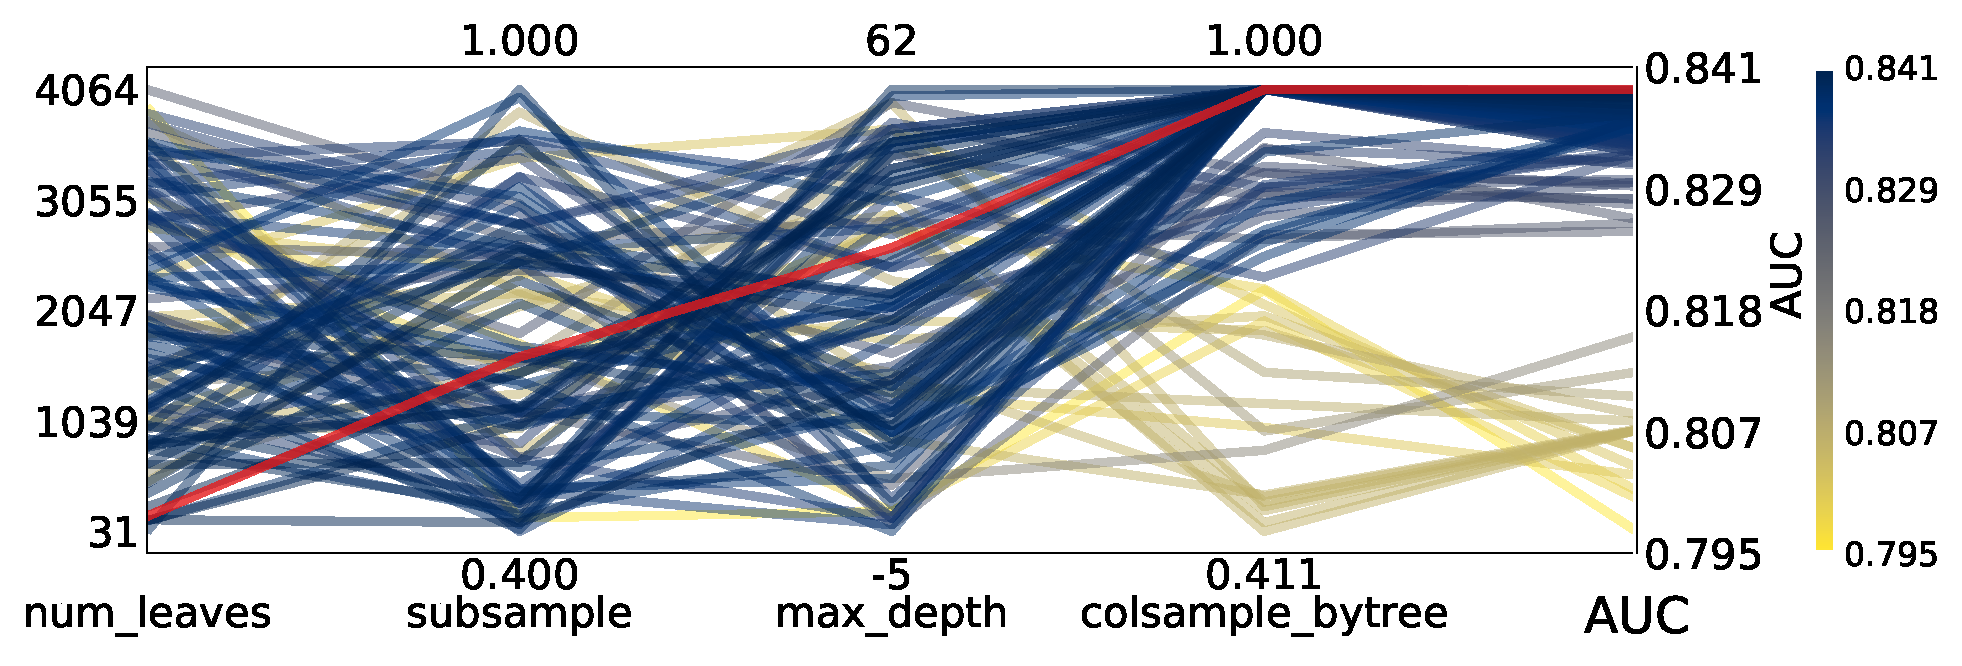
\includegraphics[width=0.98\textwidth, trim=0 0 0 0, clip]{figures/quarks/CV_viz-njet=4-name=lf_gtag_energy_ordered_lgb_down_sample=1.00-ML_vars=vertex-selection=b-ejet_min=4-n_iter_RS_lgb=99-n_iter_RS_xgb=9-cdot_cut=0.90-version=19.pdf}
  \caption[Parallel Plot of HPO Results for 4-Jet $g$-Tagging for Energy Ordered Jets]
          {Hyperparameter optimization results of $g$-tagging for 4-jet events for energy ordered jets. 
          } 
  \label{fig:q:CV_res_parallel_coords_g_tag_4j_energy_ordered}
\end{figure}


\begin{figure}[h!]
  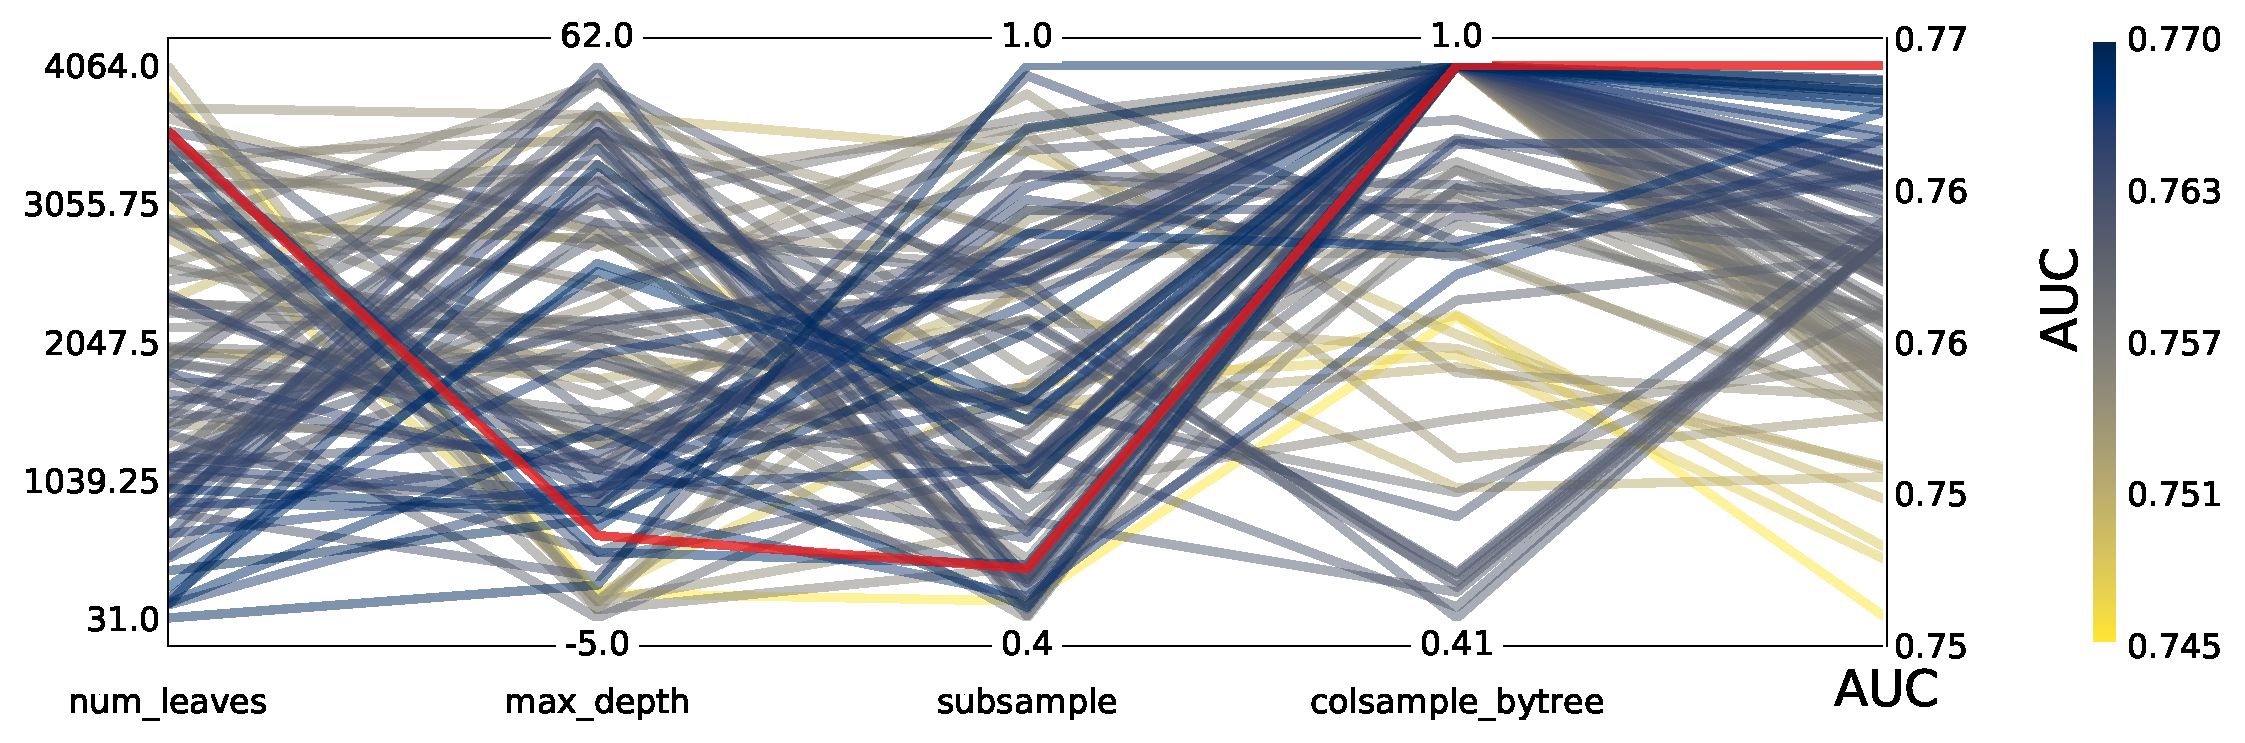
\includegraphics[width=0.98\textwidth, trim=0 0 0 0, clip]{figures/quarks/CV_viz-njet=4-name=lf_gtag_shuffled_lgb_down_sample=1.00-ML_vars=vertex-selection=b-ejet_min=4-n_iter_RS_lgb=99-n_iter_RS_xgb=9-cdot_cut=0.90-version=19.pdf}
  \caption[Parallel Plot of HPO Results for 4-Jet $g$-Tagging for Shuffled Jets]
          {Hyperparameter optimization results of $g$-tagging for 4-jet events for (row) shuffled jets. 
          } 
  \label{fig:q:CV_res_parallel_coords_g_tag_4j_shuffled}
\end{figure}

\newpage
\FloatBarrier



\begin{figure}
  \centerfloat
  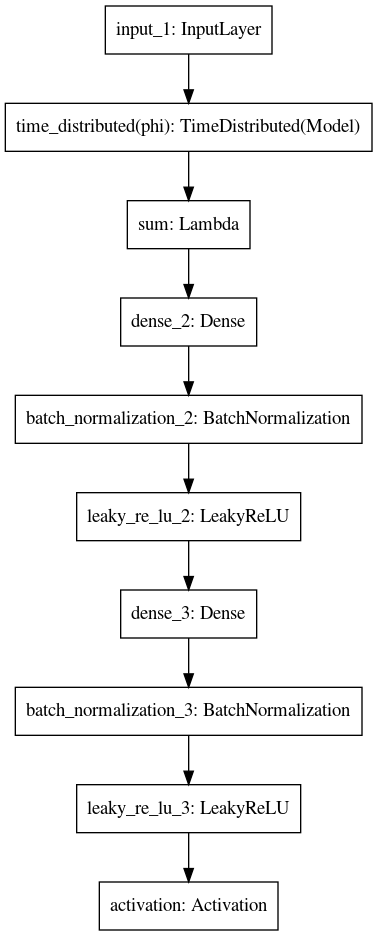
\includegraphics[width=0.5\textwidth]{figures/quarks/TensorFlow_model.png}
  \caption[PermNet Architecture]
          {Architecture of the PermNet neural network. 
          } 
  \label{fig:q:permnet_architecture}
\end{figure}

\FloatBarrier
\newpage


\begin{figure}
  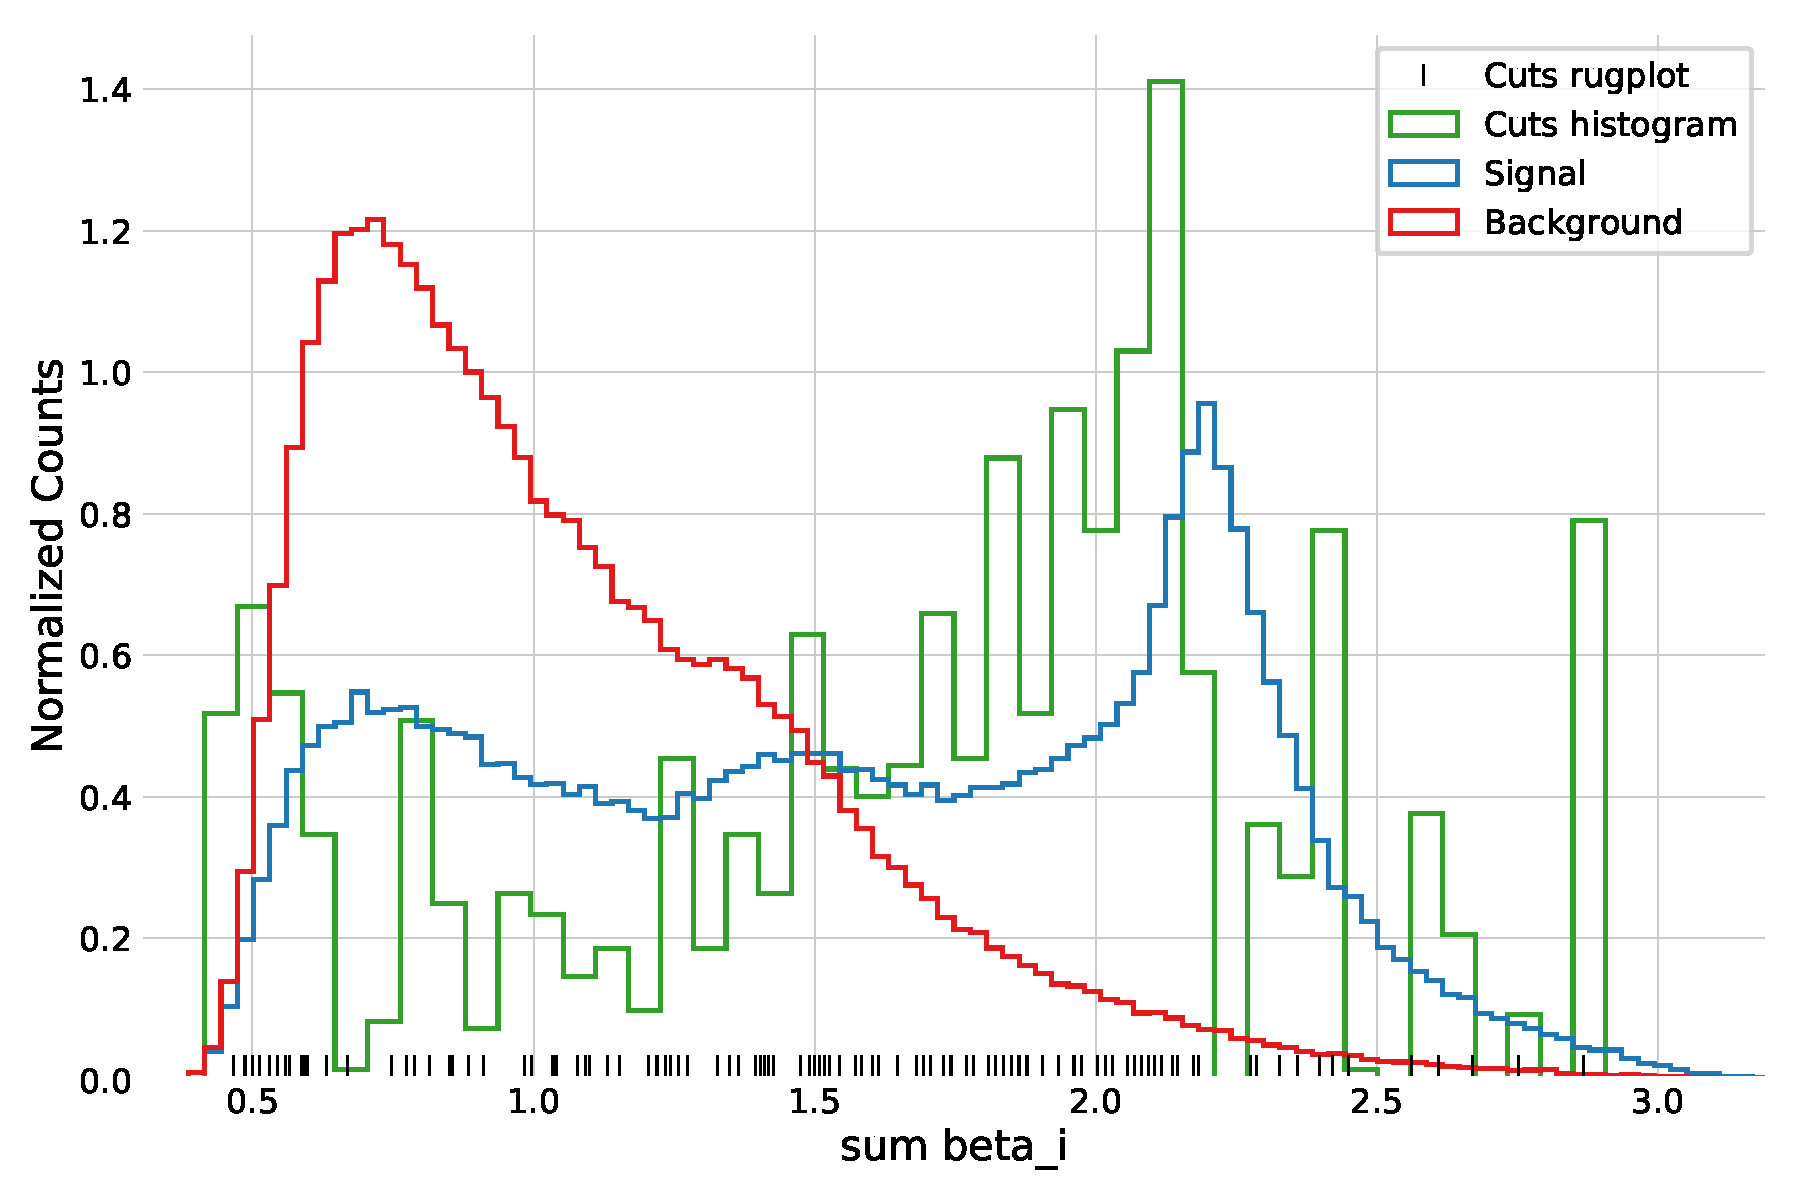
\includegraphics[width=0.95\textwidth, trim=10 10 10 20, clip]{figures/quarks/gtag_sum_method_njet=4-down_sample=1.00-ML_vars=vertex-selection=b-ejet_min=4-n_iter_RS_lgb=99-n_iter_RS_xgb=9-cdot_cut=0.90-version=19.pdf}
  \caption[1D LGB Model Cuts for 4-jets events]
          {Histogram of the distribution of \textcolor{blue}{signal} in blue and \textcolor{red}{background} in red for the 1-dimensional sum of $b$-tags for 4-jet events. A histogram of the \textcolor{green}{cut values} from the LGB model trained on this data is shown in green together with a rug plot of the cut values in black. Notice how most of the cuts match up with the signal peak at around a $\sum \beta_i \sim 2.1$.
          } 
  \label{fig:q:1d_sum_model_cuts_4j}
\end{figure}







\begin{figure}
  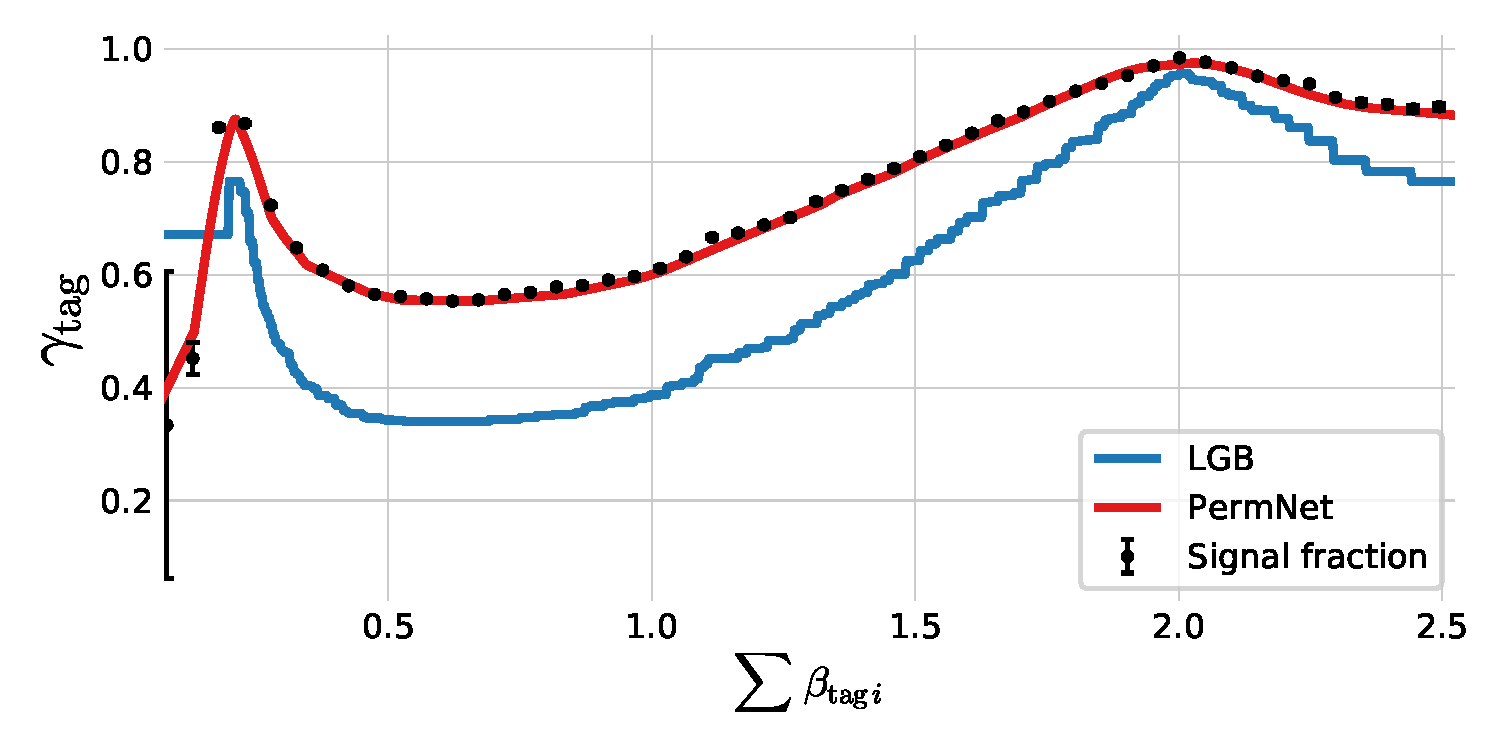
\includegraphics[width=0.95\textwidth, trim=10 10 10 10, clip]{figures/quarks/gtag_sum_models_njet=3-down_sample=1.00-ML_vars=vertex-selection=b-ejet_min=4-n_iter_RS_lgb=99-n_iter_RS_xgb=9-cdot_cut=0.90-version=19.pdf}
  \caption[1D Sum Models Predictions and Signal Fraction for 3-jets events]
          {Plot of the (1D) $g$-tag scores for 3-jet events as a function of $\sum \beta_i$ for the \textcolor{blue}{LGB} model in blue and the \textcolor{red}{PermNet} model in red. The signal fraction (based on the signal and background histograms in \figref{fig:q:1d_sum_model_cuts_3j}) is plotted as black error bars where the size of the error bars is based on the propagated uncertainties of the signal and background histogram assuming Poissonian statistics. } 
  \label{fig:q:1d_sum_models_signal_fraction_3j}
\end{figure}

\begin{figure}
  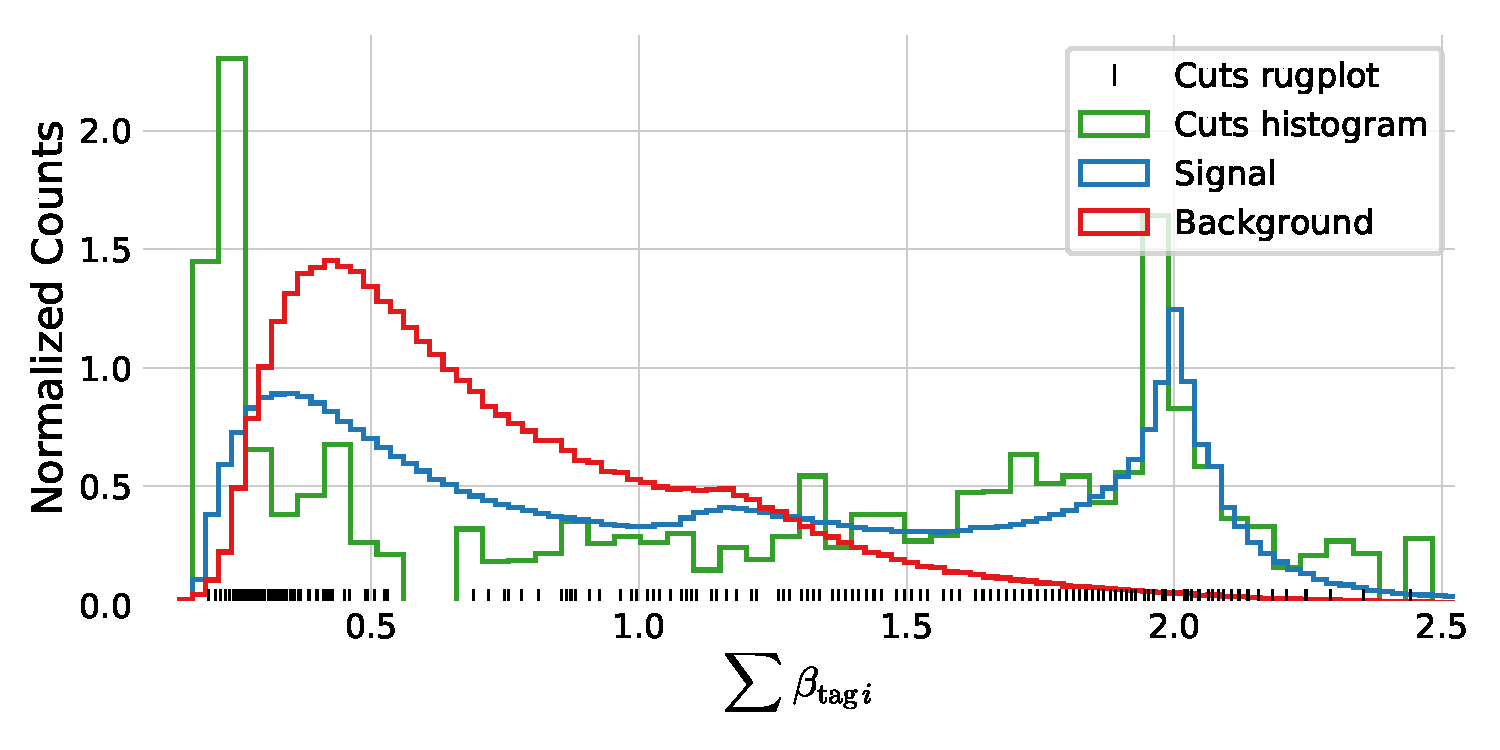
\includegraphics[width=0.95\textwidth, trim=10 10 10 20, clip]{figures/quarks/gtag_sum_method_njet=3-down_sample=1.00-ML_vars=vertex-selection=b-ejet_min=4-n_iter_RS_lgb=99-n_iter_RS_xgb=9-cdot_cut=0.90-version=19.pdf}
  \caption[1D LGB Model Cuts for 3-jets events]
          {Histogram of the distribution of \textcolor{blue}{signal} in blue and \textcolor{red}{background} in red for the 1-dimensional sum of $b$-tags for 3-jet events. A histogram of the \textcolor{green}{cut values} from the LGB model trained on this data is shown in green together with a rug plot of the cut values in black. Notice how most of the cuts match up with the signal peak at around a $\sum \beta_i \sim 2.1$.
          } 
  \label{fig:q:1d_sum_model_cuts_3j}
\end{figure}




\begin{figure}
    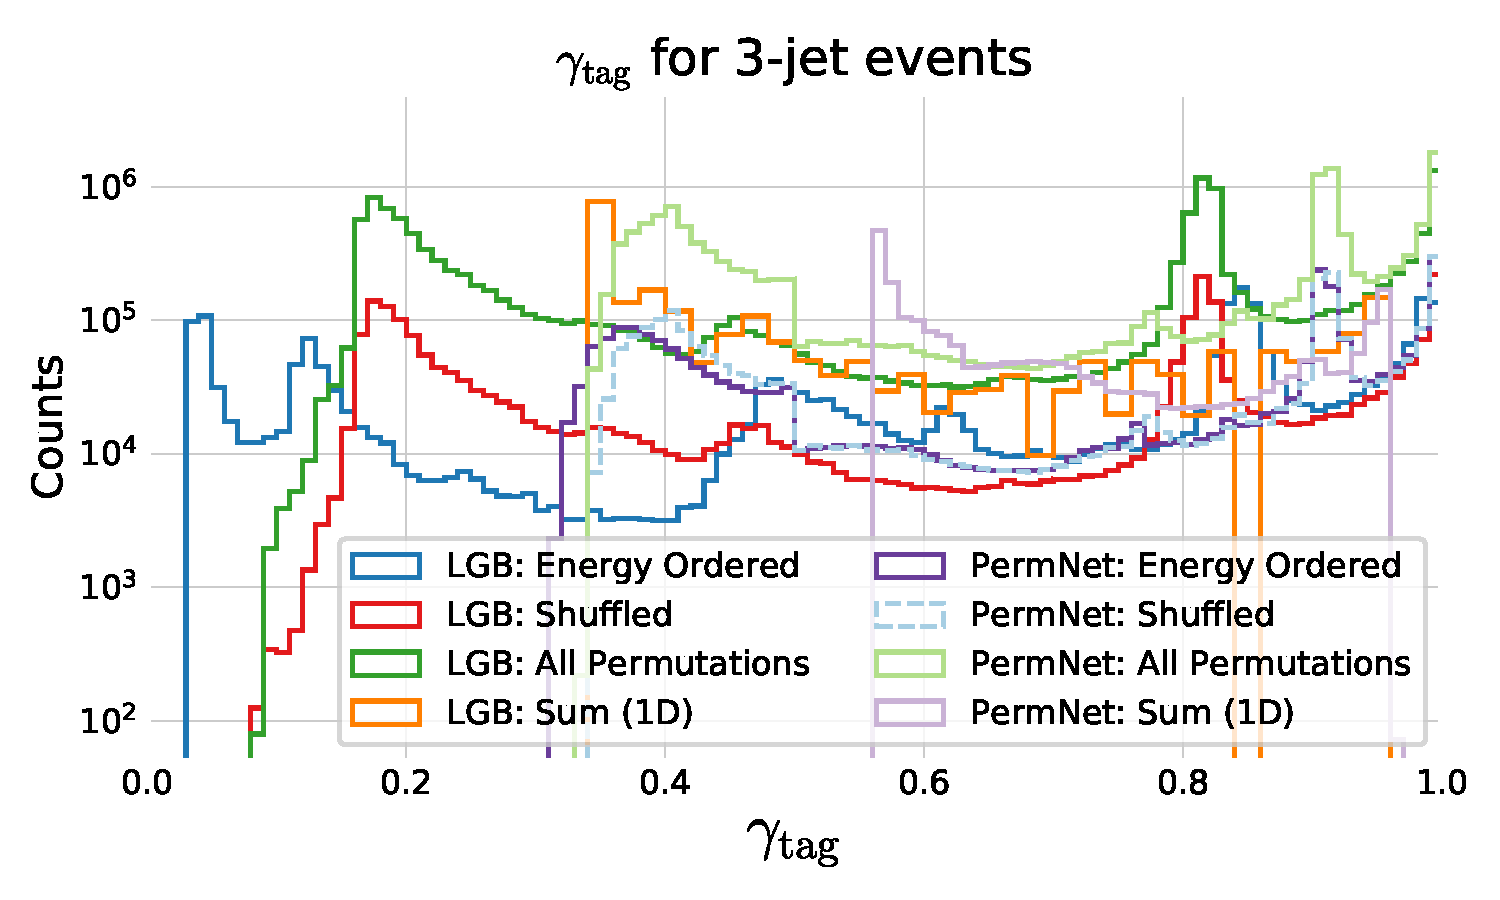
\includegraphics[width=0.95\textwidth, trim=10 10 10 45, clip]{figures/quarks/gtag_y_pred_3_jet_hist-down_sample=1.00-ML_vars=vertex-selection=b-ejet_min=4-n_iter_RS_lgb=99-n_iter_RS_xgb=9-cdot_cut=0.90-version=19.pdf}
    \caption[$g$-Tag Scores in 3-Jet Events]
            {Distribution of $g$-tag scores in 3-jet events shown with a logarithmic $y$-scale for \textcolor{blue}{LGB: Energy Ordered} in blue, \textcolor{red}{LGB: Shuffled} in red, \textcolor{green}{LGB: All Permutations} in green, \textcolor{orange}{LGB: Sum 1D} in orange, \textcolor{purple}{PermNet: Energy Ordered} in purple, \textcolor{light-blue}{PermNet: Shuffled} in light-blue, \textcolor{light-green}{PermNet: All Permutations} in light-green, \textcolor{light-purple}{PermNet: Sum 1D} in light-purple.  Here LGB and PermNet are the two different type of models and \q{Energy Ordered}, \q{Shuffled}, \q{All Permutations}, and \q{Sum 1D} are the different methods used for making the input data permutation invariant (except energy ordered).}   
    \label{fig:q:gtag_scores_3j}
  \end{figure}


  \newpage

\begin{figure}
  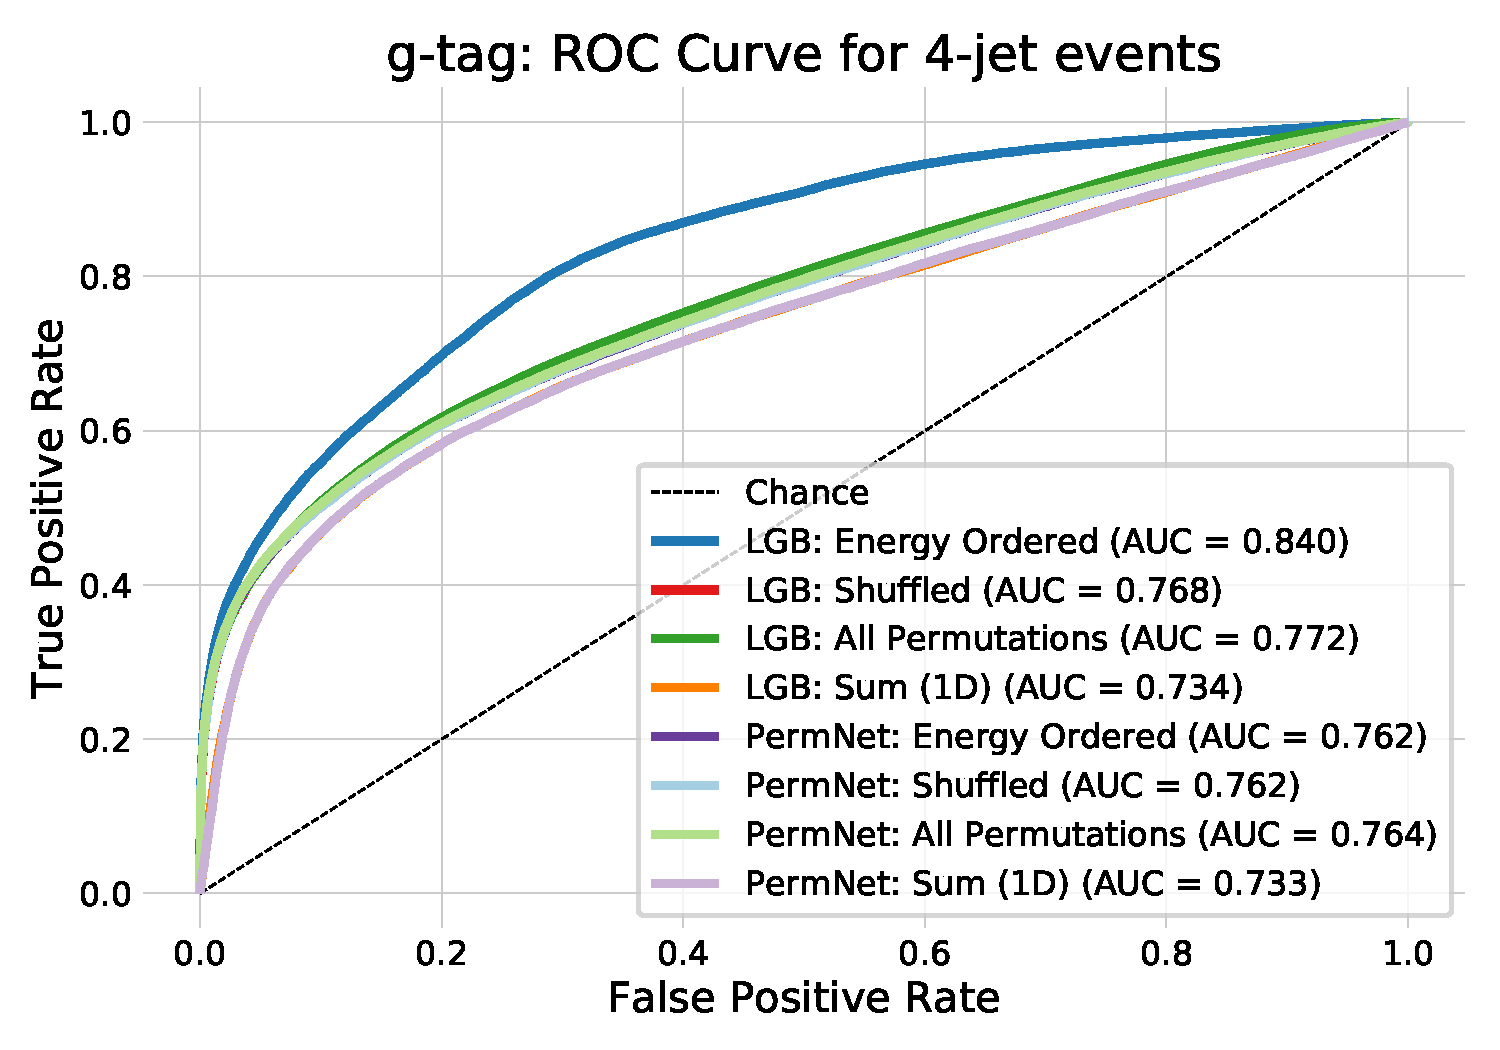
\includegraphics[width=0.95\textwidth, trim=10 10 10 40, clip]{figures/quarks/gtag_ROC_4_jet-down_sample=1.00-ML_vars=vertex-selection=b-ejet_min=4-n_iter_RS_lgb=99-n_iter_RS_xgb=9-cdot_cut=0.90-version=19.pdf}
  \caption[ROC curve for g-tag in 4-jet events]
          {ROC curve of the eight g-tag models in 4-jet events. First one in dashed black is the ROC curve that you get by random chance. The colors are the same as in \figref{fig:q:gtag_scores_4j} and in the legend also the Area Under the ROC curve (AUC) is shown. 
          Notice that the XGB model which uses the energy ordered data produced the best model, however, this model is not permutation invariant. Of the permutation invariant models (the rest), the XGB model trained on all permutations of the b-tags performs highest. The lowest performing models are the two models trained only on the 1-dimensional sum of b-tags, as expected, however, still with a better performance than expected by the author.  
          } 
  \label{fig:q:roc_gtag_4j}
\end{figure}


\begin{figure}
    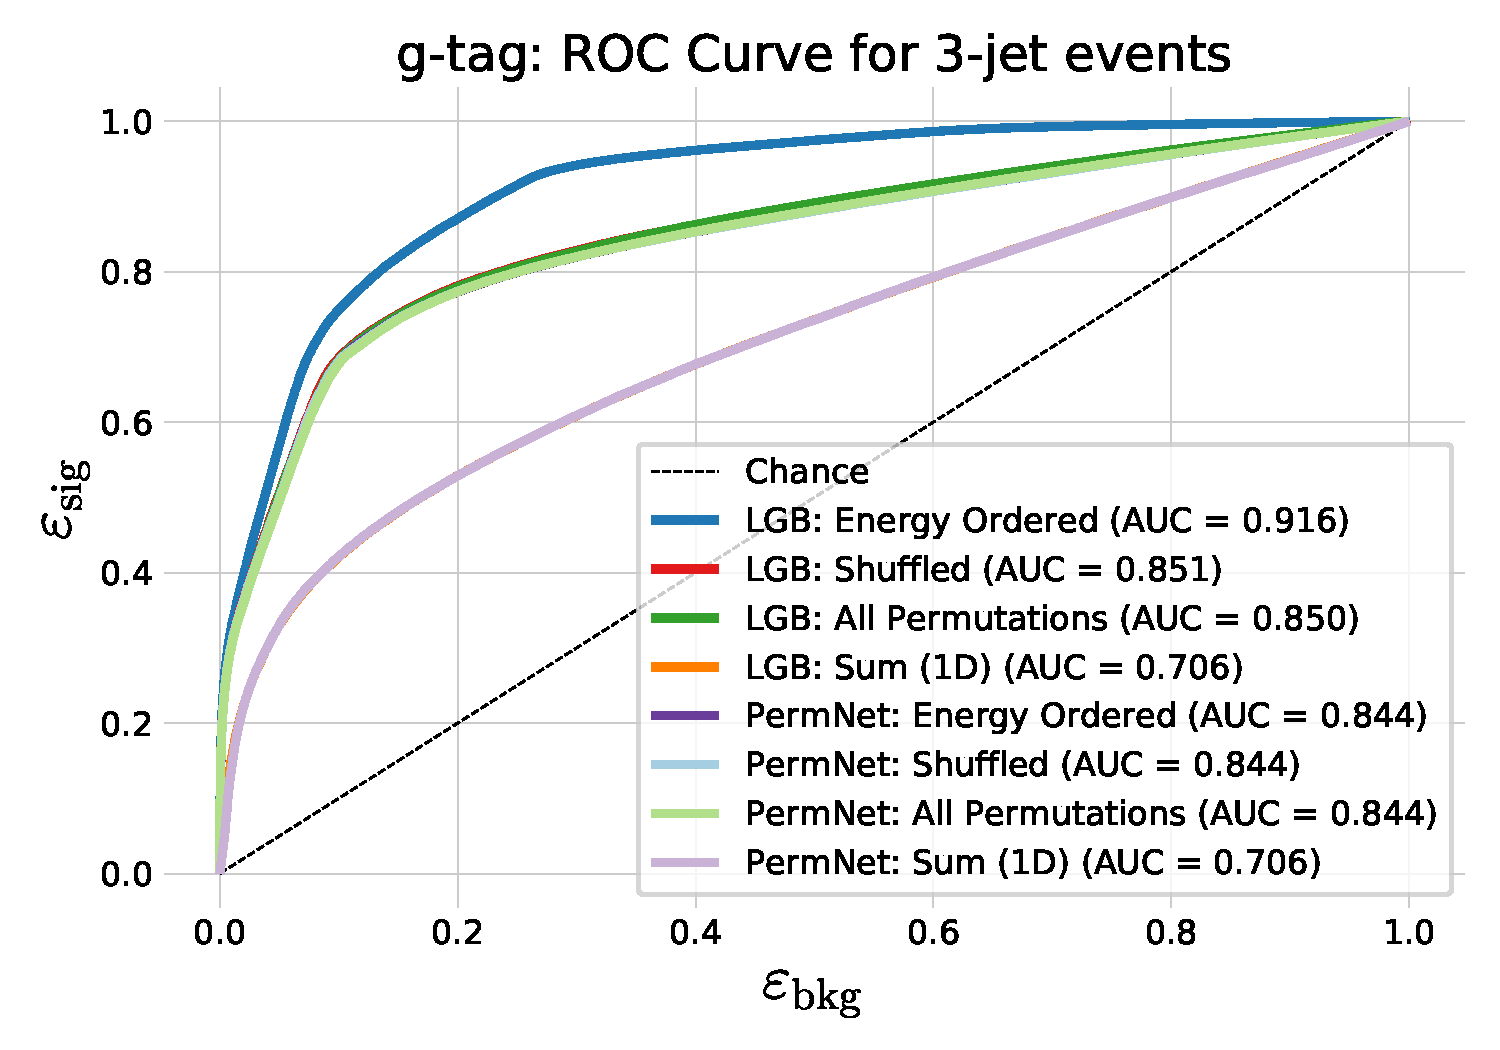
\includegraphics[width=0.95\textwidth, trim=10 10 10 40, clip]{figures/quarks/gtag_ROC_3_jet-down_sample=1.00-ML_vars=vertex-selection=b-ejet_min=4-n_iter_RS_lgb=99-n_iter_RS_xgb=9-cdot_cut=0.90-version=19.pdf}
    \caption[ROC Curve for $g$-Tag in 3-Jet Events]
            {ROC curve of the eight $g$-tag models in 3-jet. First one in dashed black is the ROC curve that you get by random chance. The colors are the same as in \figref{fig:q:gtag_scores_4j} and in the legend also the Area Under the ROC curve (AUC) is shown.} 
    \label{fig:q:roc_gtag_3j}
  \end{figure}




\begin{figure}[h!]
    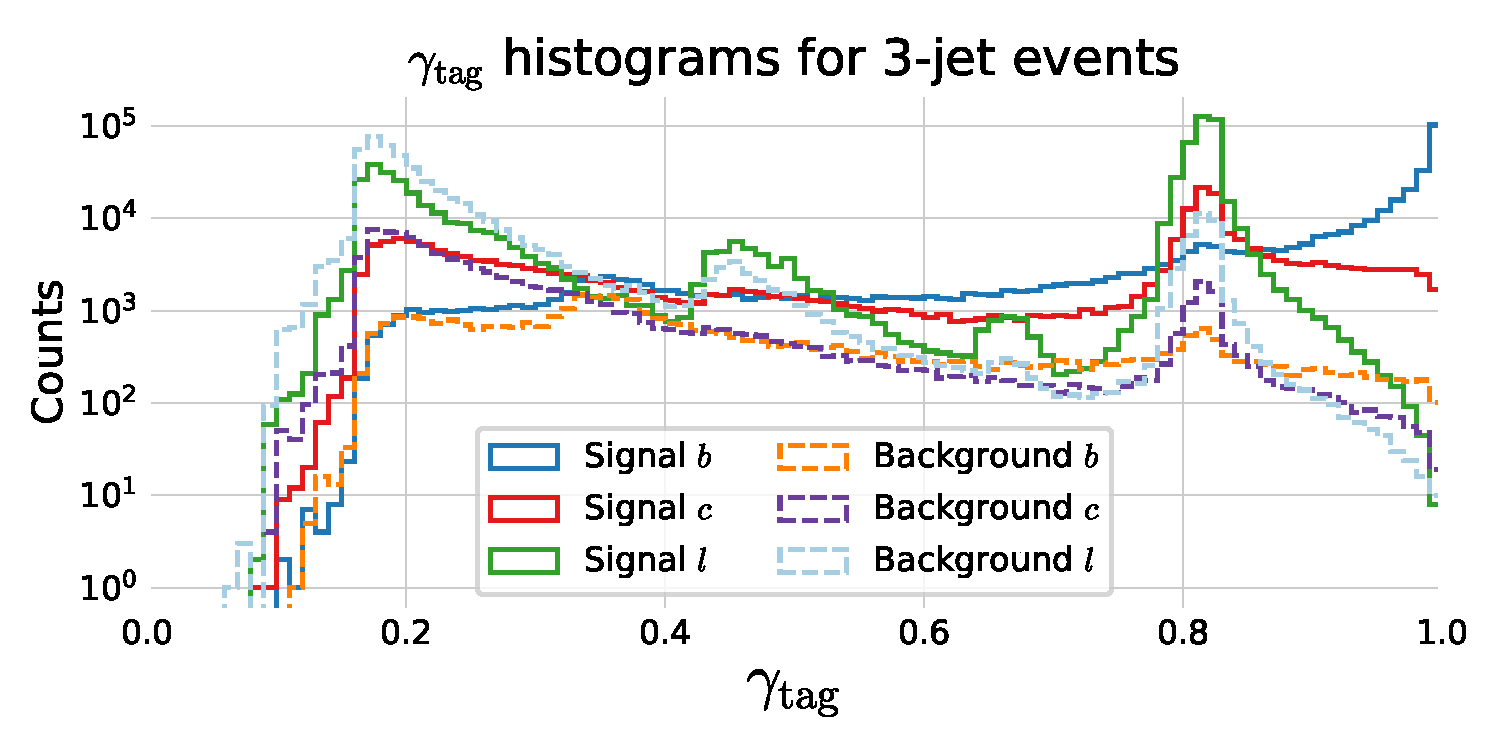
\includegraphics[width=0.95\textwidth, trim=10 10 10 45, clip]{figures/quarks/gtag-histogram-sigbkg-down_sample=1.00-ML_vars=vertex-selection=b-ejet_min=4-n_iter_RS_lgb=99-n_iter_RS_xgb=9-cdot_cut=0.90-version=19-njet=3.pdf}
    \caption[Distribution of $g$-Tag Scores in 3-Jet Events for Signal and Background]
            {Histogram of $g$-tag scores from the LGB-model in 3-jet events for \textcolor{blue}{$b$ signal} in blue, \textcolor{red}{$c$ signal} in red, \textcolor{green}{$l$ ($uds$) signal} in green, \textcolor{orange}{$b$ background} in orange, \textcolor{purple}{$c$ background} in purple, \textcolor{light-blue}{$l$ ($uds$) background} in light-blue.
            } 
    \label{fig:q:gtag_scores_3j_sig_bkg}
  \end{figure}



\begin{table}[]
    \centerfloat
    \begin{tabular}{@{}rccc@{}}
    ${\beta_\mathrm{tag}}_i$  & Energy Ordered & Shuffled & All Permutations \\ \midrule
  1 & $ 0.827 \pm 0.006 $  &  $ 0.924 \pm 0.006 $  &  $ 0.923 \pm 0.006 $  \\
  2 & $ 0.749 \pm 0.006 $  &  $ 0.909 \pm 0.006 $  &  $ 0.918 \pm 0.005 $  \\
  3 & $ 1.198 \pm 0.006 $  &  $ 0.878 \pm 0.005 $  &  $ 0.906 \pm 0.005 $  \\
  \end{tabular}
  \caption[Global SHAP Feature Importances for the $g$-Tagging Models in 3-Jet Events]{Global SHAP feature importances $\phi^\mathrm{tot}_{\beta_\mathrm{i}}$ for the three $g$-Tagging Models in 3-Jet Events. Each $\phi^\mathrm{tot}_{\beta_\mathrm{i}}$ is shown for the three methods in the columns and the three $b$-tags as variables in the rows.}
  \label{table:q:shap_g_taggging_global_3j}
\end{table}



\begin{figure}
  \centerfloat
  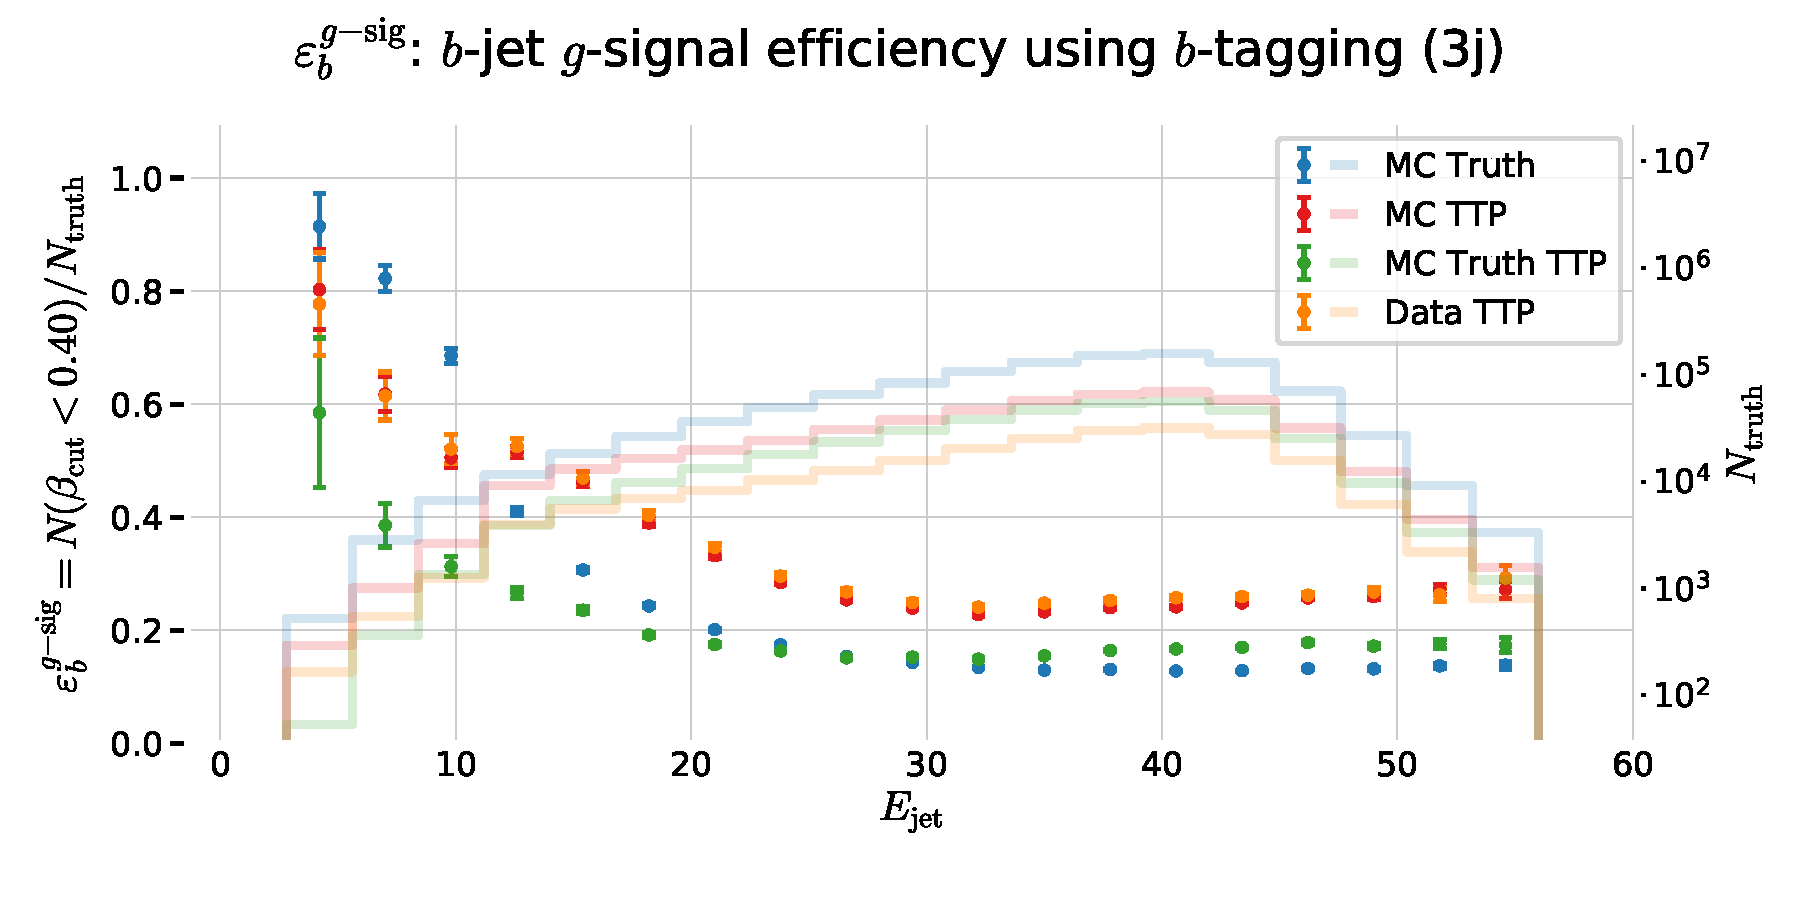
\includegraphics[width=1.1\textwidth, trim=20 30 0 40, clip]{figures/quarks/eff_b_gsig-down_sample=1.00-ML_vars=vertex-selection=b-ejet_min=4-n_iter_RS_lgb=99-n_iter_RS_xgb=9-cdot_cut=0.90-version=19.pdf}
  \caption[$b$-Tagging Efficiency $\varepsilon_b^{g\dash\mathrm{sig}}$ as a Function of Jet Energy]
          {$b$-tag efficiency for $b$-jets in the $g$-signal region for 3-jet events, $\varepsilon_b^{g\dash\mathrm{sig}}$, as a function of jet energy $E_\mathrm{jet}$. In the plot the efficiencies are shown for \textcolor{blue}{MC TTP} in blue, \textcolor{red}{Data TTP} in red, \textcolor{green}{MC Truth TTP} in green, and \textcolor{orange}{MC Truth TTP} in orange. The efficiencies (the errorbars) can be read off on the left $y$-axis and the counts (histograms) on the right $y$-axis.} 
  \label{fig:q:effiency_btag_bjet_gsig}
\end{figure}


\begin{figure}
  \centerfloat
  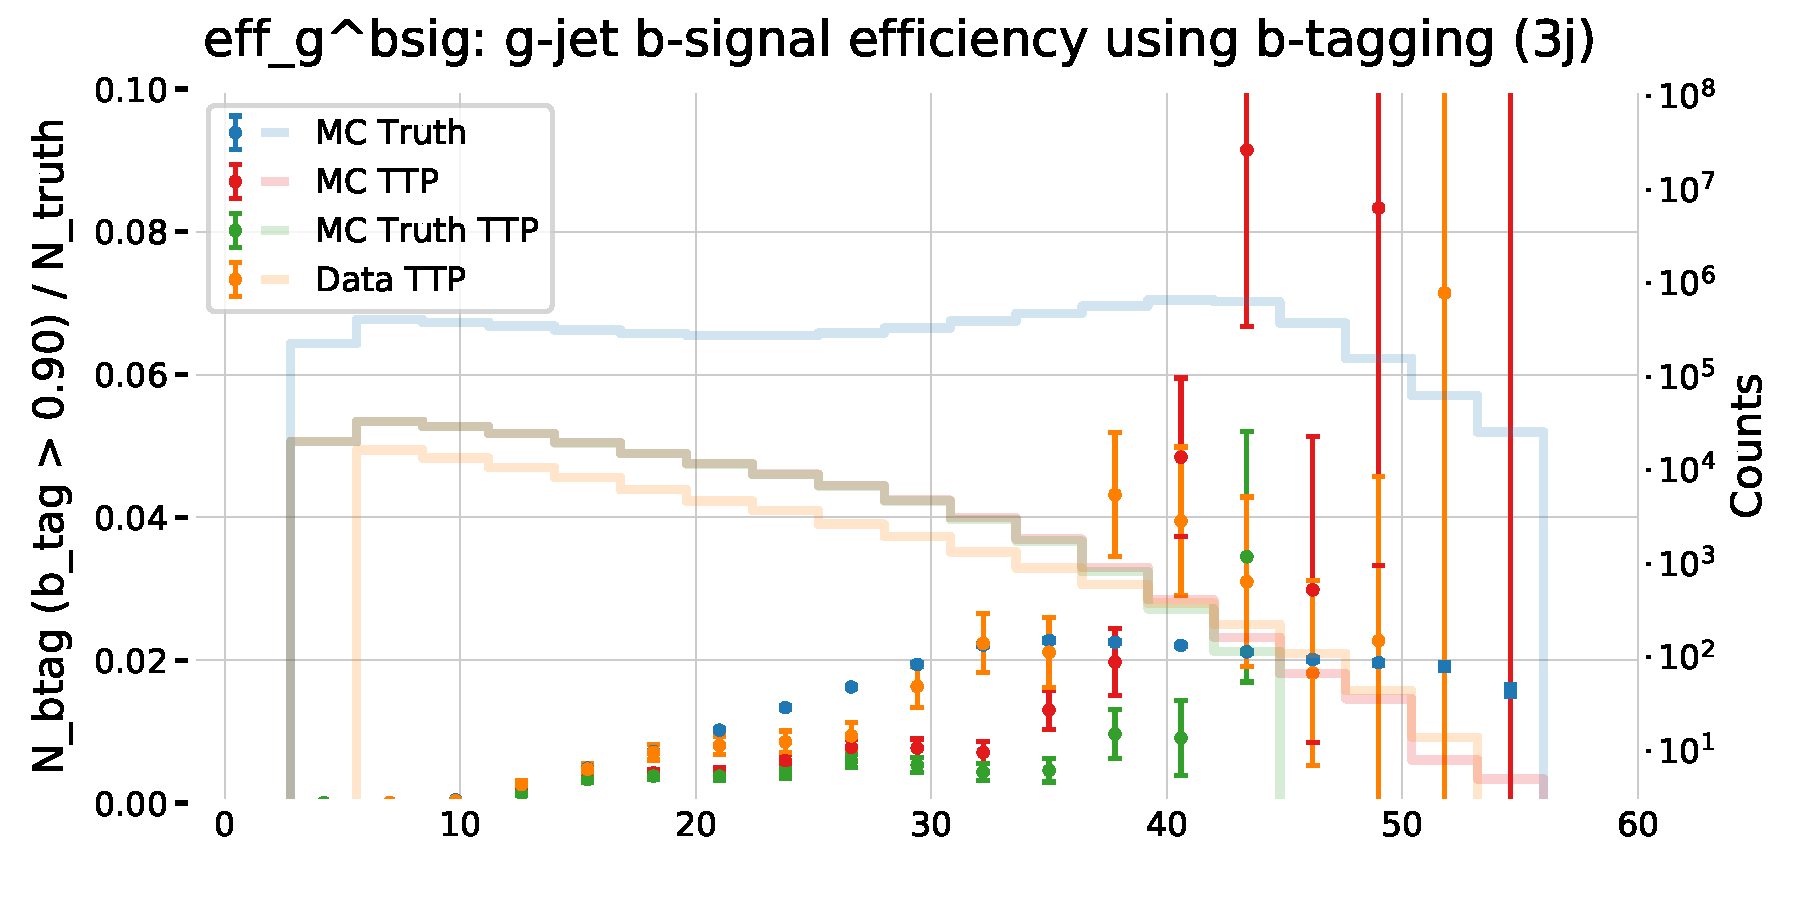
\includegraphics[width=1.1\textwidth, trim=20 30 0 40, clip]{figures/quarks/eff_g_bsig-down_sample=1.00-ML_vars=vertex-selection=b-ejet_min=4-n_iter_RS_lgb=99-n_iter_RS_xgb=9-cdot_cut=0.90-version=19.pdf}
  \caption[$b$-Tagging Efficiency $\varepsilon_g^{b\dash\mathrm{sig}}$ as a Function of Jet Energy]
          {$b$-tag efficiency for $g$-jets in the $b$-signal region for 3-jet events, $\varepsilon_g^{b\dash\mathrm{sig}}$, as a function of jet energy $E_\mathrm{jet}$. In the plot the efficiencies are shown for \textcolor{blue}{MC TTP} in blue, \textcolor{red}{Data TTP} in red, \textcolor{green}{MC Truth TTP} in green, and \textcolor{orange}{MC Truth TTP} in orange. The efficiencies (the errorbars) can be read off on the left $y$-axis and the counts (histograms) on the right $y$-axis.} 
  \label{fig:q:effiency_btag_gjet_bsig}
\end{figure}


\FloatBarrier
\newpage

\begin{figure}[h!]
  \centerfloat
  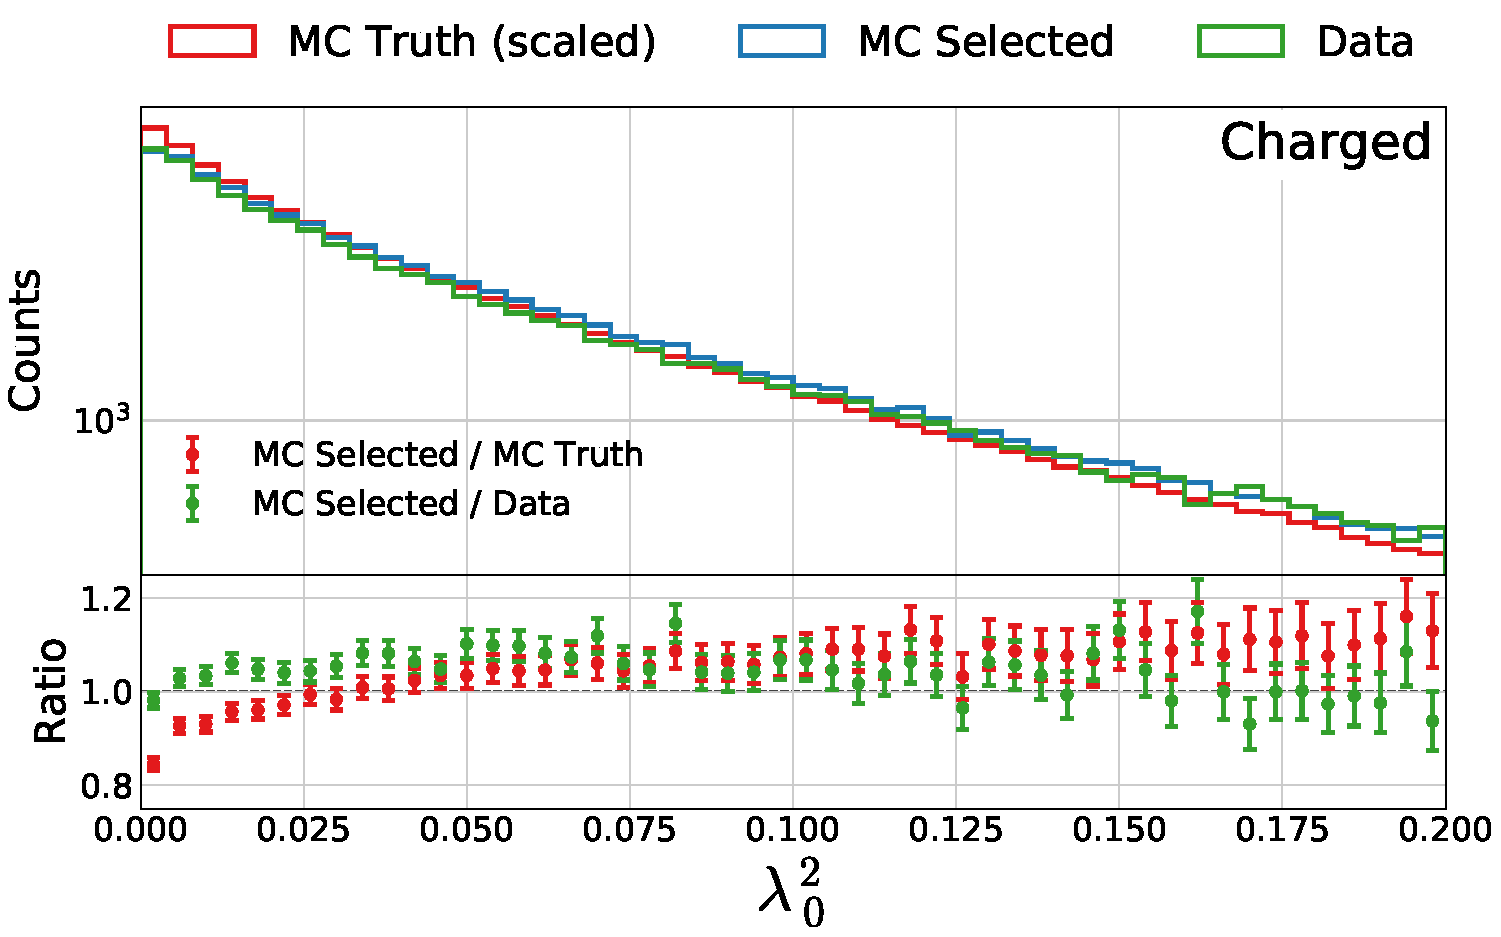
\includegraphics[width=0.99\textwidth, trim=0 0 0 0, clip, page=1]{figures/quarks/generalized_angularities_cha-down_sample=1.00-ML_vars=vertex-selection=b-ejet_min=4-n_iter_RS_lgb=99-n_iter_RS_xgb=9-cdot_cut=0.90-version=19.pdf}
  \caption[Generalized Angularities for Charged Gluons Jets in 3-Jet Events: $\lambda_0^2$]
          {Distribution of the generalized angularity $\lambda_0^2$ for charged gluons jets in 3-jet events. The distributions for \textcolor{red}{MC Truth} is shown in red, \textcolor{blue}{MC Truth} in blue, and \textcolor{green}{Data} in green in the top plot and in the bottom plot the ratio between \textcolor{red}{MC Selected and MC Truth} is shown in red and between \textcolor{green}{MC Selected and Data} in green. }
  \label{fig:q:generalized_angularities_cha_lambda_0_2}
\end{figure}
\begin{figure}[h!]
  \centerfloat
  \includegraphics[width=0.99\textwidth, trim=0 0 0 0, clip, page=2]{figures/quarks/generalized_angularities_cha-down_sample=1.00-ML_vars=vertex-selection=b-ejet_min=4-n_iter_RS_lgb=99-n_iter_RS_xgb=9-cdot_cut=0.90-version=19.pdf}
  \caption[Generalized Angularities for Charged Gluons Jets in 3-Jet Events: $\lambda_{\frac{1}{2}}^1$]
          {Distribution of the generalized angularity $\lambda_{\frac{1}{2}}^1$ for charged gluons jets in 3-jet events. The distributions for \textcolor{red}{MC Truth} is shown in red, \textcolor{blue}{MC Truth} in blue, and \textcolor{green}{Data} in green in the top plot and in the bottom plot the ratio between \textcolor{red}{MC Selected and MC Truth} is shown in red and between \textcolor{green}{MC Selected and Data} in green. }
  \label{fig:q:generalized_angularities_cha_lambda_5_1}
\end{figure}
\begin{figure}[h!]
  \centerfloat
  \includegraphics[width=0.99\textwidth, trim=0 0 0 0, clip, page=3]{figures/quarks/generalized_angularities_cha-down_sample=1.00-ML_vars=vertex-selection=b-ejet_min=4-n_iter_RS_lgb=99-n_iter_RS_xgb=9-cdot_cut=0.90-version=19.pdf}
  \caption[Generalized Angularities for Charged Gluons Jets in 3-Jet Events: $\lambda_1^1$]
          {Distribution of the generalized angularity $\lambda_1^1$ for charged gluons jets in 3-jet events. The distributions for \textcolor{red}{MC Truth} is shown in red, \textcolor{blue}{MC Truth} in blue, and \textcolor{green}{Data} in green in the top plot and in the bottom plot the ratio between \textcolor{red}{MC Selected and MC Truth} is shown in red and between \textcolor{green}{MC Selected and Data} in green. }
  \label{fig:q:generalized_angularities_cha_lambda_1_1}
\end{figure}
\begin{figure}[h!]
  \centerfloat
  \includegraphics[width=0.99\textwidth, trim=0 0 0 0, clip, page=4]{figures/quarks/generalized_angularities_cha-down_sample=1.00-ML_vars=vertex-selection=b-ejet_min=4-n_iter_RS_lgb=99-n_iter_RS_xgb=9-cdot_cut=0.90-version=19.pdf}
  \caption[Generalized Angularities for Charged Gluons Jets in 3-Jet Events: $\lambda_1^2$]
          {Distribution of the generalized angularity $\lambda_1^2$ for charged gluons jets in 3-jet events. The distributions for \textcolor{red}{MC Truth} is shown in red, \textcolor{blue}{MC Truth} in blue, and \textcolor{green}{Data} in green in the top plot and in the bottom plot the ratio between \textcolor{red}{MC Selected and MC Truth} is shown in red and between \textcolor{green}{MC Selected and Data} in green. }
  \label{fig:q:generalized_angularities_cha_lambda_1_2}
\end{figure}
\begin{figure}[h!]
  \centerfloat
  \includegraphics[width=0.99\textwidth, trim=0 0 0 0, clip, page=5]{figures/quarks/generalized_angularities_cha-down_sample=1.00-ML_vars=vertex-selection=b-ejet_min=4-n_iter_RS_lgb=99-n_iter_RS_xgb=9-cdot_cut=0.90-version=19.pdf}
  \caption[Generalized Angularities for Charged Gluons Jets in 3-Jet Events: $\lambda_0^0$]
          {Distribution of the generalized angularity $\lambda_0^0$ for charged gluons jets in 3-jet events. The distributions for \textcolor{red}{MC Truth} is shown in red, \textcolor{blue}{MC Truth} in blue, and \textcolor{green}{Data} in green in the top plot and in the bottom plot the ratio between \textcolor{red}{MC Selected and MC Truth} is shown in red and between \textcolor{green}{MC Selected and Data} in green. }
  \label{fig:q:generalized_angularities_cha_lambda_0_0}
\end{figure}


\begin{figure}[h!]
  \centerfloat
  \includegraphics[width=0.99\textwidth, trim=0 0 0 0, clip, page=6]{figures/quarks/generalized_angularities_cha-down_sample=1.00-ML_vars=vertex-selection=b-ejet_min=4-n_iter_RS_lgb=99-n_iter_RS_xgb=9-cdot_cut=0.90-version=19.pdf}
  \caption[Generalized Angularities for Neutral Gluons Jets in 3-Jet Events: $\lambda_0^2$]
          {Distribution of the generalized angularity $\lambda_0^2$ for charged gluons jets in 3-jet events. The distributions for \textcolor{red}{MC Truth} is shown in red, \textcolor{blue}{MC Truth} in blue, and \textcolor{green}{Data} in green in the top plot and in the bottom plot the ratio between \textcolor{red}{MC Selected and MC Truth} is shown in red and between \textcolor{green}{MC Selected and Data} in green. }
  \label{fig:q:generalized_angularities_neu_lambda_0_2}
\end{figure}
\begin{figure}[h!]
  \centerfloat
  \includegraphics[width=0.99\textwidth, trim=0 0 0 0, clip, page=7]{figures/quarks/generalized_angularities_cha-down_sample=1.00-ML_vars=vertex-selection=b-ejet_min=4-n_iter_RS_lgb=99-n_iter_RS_xgb=9-cdot_cut=0.90-version=19.pdf}
  \caption[Generalized Angularities for Neutral Gluons Jets in 3-Jet Events: $\lambda_{\frac{1}{2}}^1$]
          {Distribution of the generalized angularity $\lambda_{\frac{1}{2}}^1$ for neutral gluons clusters in 3-jet events. The distributions for \textcolor{red}{MC Truth} is shown in red, \textcolor{blue}{MC Truth} in blue, and \textcolor{green}{Data} in green in the top plot and in the bottom plot the ratio between \textcolor{red}{MC Selected and MC Truth} is shown in red and between \textcolor{green}{MC Selected and Data} in green. }
  \label{fig:q:generalized_angularities_neu_lambda_5_1}
\end{figure}
\begin{figure}[h!]
  \centerfloat
  \includegraphics[width=0.99\textwidth, trim=0 0 0 0, clip, page=8]{figures/quarks/generalized_angularities_cha-down_sample=1.00-ML_vars=vertex-selection=b-ejet_min=4-n_iter_RS_lgb=99-n_iter_RS_xgb=9-cdot_cut=0.90-version=19.pdf}
  \caption[Generalized Angularities for Neutral Gluons Jets in 3-Jet Events: $\lambda_1^1$]
          {Distribution of the generalized angularity $\lambda_1^1$ for neutral gluons clusters in 3-jet events. The distributions for \textcolor{red}{MC Truth} is shown in red, \textcolor{blue}{MC Truth} in blue, and \textcolor{green}{Data} in green in the top plot and in the bottom plot the ratio between \textcolor{red}{MC Selected and MC Truth} is shown in red and between \textcolor{green}{MC Selected and Data} in green. }
  \label{fig:q:generalized_angularities_neu_lambda_1_1}
\end{figure}
\begin{figure}[h!]
  \centerfloat
  \includegraphics[width=0.99\textwidth, trim=0 0 0 0, clip, page=9]{figures/quarks/generalized_angularities_cha-down_sample=1.00-ML_vars=vertex-selection=b-ejet_min=4-n_iter_RS_lgb=99-n_iter_RS_xgb=9-cdot_cut=0.90-version=19.pdf}
  \caption[Generalized Angularities for Neutral Gluons Jets in 3-Jet Events: $\lambda_1^2$]
          {Distribution of the generalized angularity $\lambda_1^2$ for neutral gluons clusters in 3-jet events. The distributions for \textcolor{red}{MC Truth} is shown in red, \textcolor{blue}{MC Truth} in blue, and \textcolor{green}{Data} in green in the top plot and in the bottom plot the ratio between \textcolor{red}{MC Selected and MC Truth} is shown in red and between \textcolor{green}{MC Selected and Data} in green. }
  \label{fig:q:generalized_angularities_neu_lambda_1_2}
\end{figure}
\begin{figure}[h!]
  \centerfloat
  \includegraphics[width=0.99\textwidth, trim=0 0 0 0, clip, page=10]{figures/quarks/generalized_angularities_cha-down_sample=1.00-ML_vars=vertex-selection=b-ejet_min=4-n_iter_RS_lgb=99-n_iter_RS_xgb=9-cdot_cut=0.90-version=19.pdf}
  \caption[Generalized Angularities for Neutral Gluons Jets in 3-Jet Events: $\lambda_0^0$]
          {Distribution of the generalized angularity $\lambda_0^0$ for neutral gluons clusters in 3-jet events. The distributions for \textcolor{red}{MC Truth} is shown in red, \textcolor{blue}{MC Truth} in blue, and \textcolor{green}{Data} in green in the top plot and in the bottom plot the ratio between \textcolor{red}{MC Selected and MC Truth} is shown in red and between \textcolor{green}{MC Selected and Data} in green. }
  \label{fig:q:generalized_angularities_neu_lambda_0_0}
\end{figure}











\FloatBarrier
\newpage

\begin{figure}
  \centerfloat
  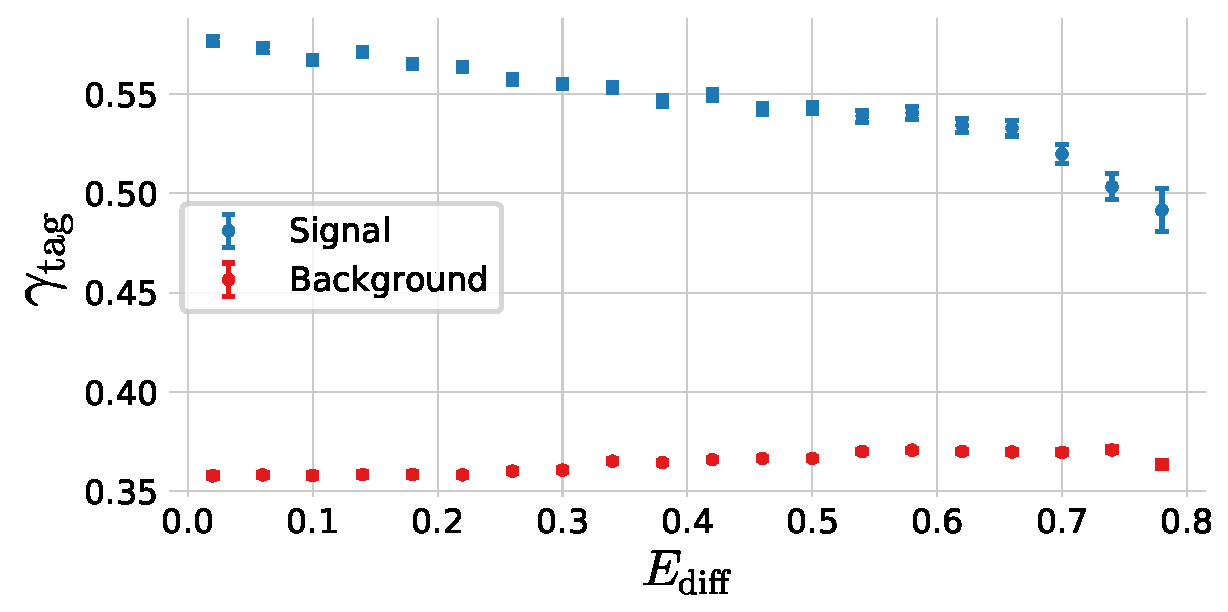
\includegraphics[width=0.99\textwidth, trim=0 0 0 0, clip, page=1]{figures/quarks/gtag-g_splitting_gtag_errorbar-down_sample=1.00-ML_vars=vertex-selection=b-ejet_min=4-n_iter_RS_lgb=99-n_iter_RS_xgb=9-cdot_cut=0.90-version=19-njet=4.pdf}
  \caption[Relationship Between the $g$-Tag Value $\gamma_\mathrm{tag}$ and the Gluon Splitting Variable $E_\mathrm{diff}$]
          {Relationship between the $g$-tag value $\gamma_\mathrm{tag}$ and the gluon splitting variable $E_\mathrm{diff}$. The \textcolor{blue}{signal events} (according to MC Truth) are plotted in blue and \textcolor{red}{background events} (according to MC Truth) in red. 
          } 
  \label{fig:q:gtag_gluon_splitting_variable_E_diff}
\end{figure}
\begin{figure}
  \centerfloat
  \includegraphics[width=0.99\textwidth, trim=0 0 0 0, clip, page=2]{figures/quarks/gtag-g_splitting_gtag_errorbar-down_sample=1.00-ML_vars=vertex-selection=b-ejet_min=4-n_iter_RS_lgb=99-n_iter_RS_xgb=9-cdot_cut=0.90-version=19-njet=4.pdf}
  \caption[Relationship Between the $g$-Tag Value $\gamma_\mathrm{tag}$ and the Gluon Splitting Variable $E_{\mathrm{rel}_\mathrm{min}}$]
          {Relationship between the $g$-tag value $\gamma_\mathrm{tag}$ and the gluon splitting variable $E_{\mathrm{rel}_\mathrm{min}}$. The \textcolor{blue}{signal events} (according to MC Truth) are plotted in blue and \textcolor{red}{background events} (according to MC Truth) in red. 
          } 
  \label{fig:q:gtag_gluon_splitting_variable_E_rel_min}
\end{figure}
\begin{figure}
  \centerfloat
  \includegraphics[width=0.99\textwidth, trim=0 0 0 0, clip, page=3]{figures/quarks/gtag-g_splitting_gtag_errorbar-down_sample=1.00-ML_vars=vertex-selection=b-ejet_min=4-n_iter_RS_lgb=99-n_iter_RS_xgb=9-cdot_cut=0.90-version=19-njet=4.pdf}
  \caption[Relationship Between the $g$-Tag Value $\gamma_\mathrm{tag}$ and the Gluon Splitting Variable $E_\mathrm{rel}$]
          {Relationship between the $g$-tag value $\gamma_\mathrm{tag}$ and the gluon splitting variable $E_\mathrm{rel}$. The \textcolor{blue}{signal events} (according to MC Truth) are plotted in blue and \textcolor{red}{background events} (according to MC Truth) in red. 
          } 
  \label{fig:q:gtag_gluon_splitting_variable_E_rel}
\end{figure}
\begin{figure}
  \centerfloat
  \includegraphics[width=0.99\textwidth, trim=0 0 0 0, clip, page=4]{figures/quarks/gtag-g_splitting_gtag_errorbar-down_sample=1.00-ML_vars=vertex-selection=b-ejet_min=4-n_iter_RS_lgb=99-n_iter_RS_xgb=9-cdot_cut=0.90-version=19-njet=4.pdf}
  \caption[Relationship Between the $g$-Tag Value $\gamma_\mathrm{tag}$ and the Gluon Splitting Variable $\Delta_\theta$]
          {Relationship between the $g$-tag value $\gamma_\mathrm{tag}$ and the gluon splitting variable $\Delta_\theta$. The \textcolor{blue}{signal events} (according to MC Truth) are plotted in blue and \textcolor{red}{background events} (according to MC Truth) in red. 
          } 
  \label{fig:q:gtag_gluon_splitting_variable_delta_theta}
\end{figure}
\begin{figure}
  \centerfloat
  \includegraphics[width=0.99\textwidth, trim=0 0 0 0, clip, page=5]{figures/quarks/gtag-g_splitting_gtag_errorbar-down_sample=1.00-ML_vars=vertex-selection=b-ejet_min=4-n_iter_RS_lgb=99-n_iter_RS_xgb=9-cdot_cut=0.90-version=19-njet=4.pdf}
  \caption[Relationship Between the $g$-Tag Value $\gamma_\mathrm{tag}$ and the Gluon Splitting Variable $m_{gg}$]
          {Relationship between the $g$-tag value $\gamma_\mathrm{tag}$ and the gluon splitting variable $m_{gg}$. The \textcolor{blue}{signal events} (according to MC Truth) are plotted in blue and \textcolor{red}{background events} (according to MC Truth) in red. 
          } 
  \label{fig:q:gtag_gluon_splitting_variable_m_gg}
\end{figure}
\begin{figure}
  \centerfloat
  \includegraphics[width=0.99\textwidth, trim=0 0 0 0, clip, page=6]{figures/quarks/gtag-g_splitting_gtag_errorbar-down_sample=1.00-ML_vars=vertex-selection=b-ejet_min=4-n_iter_RS_lgb=99-n_iter_RS_xgb=9-cdot_cut=0.90-version=19-njet=4.pdf}
  \caption[Relationship Between the $g$-Tag Value $\gamma_\mathrm{tag}$ and the Gluon Splitting Variable $\phi_\mathrm{\parallel}$]
          {Relationship between the $g$-tag value $\gamma_\mathrm{tag}$ and the gluon splitting variable $\phi_\mathrm{\parallel}$. The \textcolor{blue}{signal events} (according to MC Truth) are plotted in blue and \textcolor{red}{background events} (according to MC Truth) in red. 
          } 
  \label{fig:q:gtag_gluon_splitting_variable_phi_planes}
\end{figure}
\begin{figure}
  \centerfloat
  \includegraphics[width=0.99\textwidth, trim=0 0 0 0, clip, page=7]{figures/quarks/gtag-g_splitting_gtag_errorbar-down_sample=1.00-ML_vars=vertex-selection=b-ejet_min=4-n_iter_RS_lgb=99-n_iter_RS_xgb=9-cdot_cut=0.90-version=19-njet=4.pdf}
  \caption[Relationship Between the $g$-Tag Value $\gamma_\mathrm{tag}$ and the Gluon Splitting Variable $\ln \left( k_t^2 / m_\mathrm{vis}^2 \right)$]
          {Relationship between the $g$-tag value $\gamma_\mathrm{tag}$ and the gluon splitting variable $\ln \left( k_t^2 / m_\mathrm{vis}^2 \right)$. The \textcolor{blue}{signal events} (according to MC Truth) are plotted in blue and \textcolor{red}{background events} (according to MC Truth) in red. 
          } 
  \label{fig:q:gtag_gluon_splitting_variable_ln_kt_m_vis}
\end{figure}
\begin{figure}
  \centerfloat
  \includegraphics[width=0.99\textwidth, trim=0 0 0 0, clip, page=8]{figures/quarks/gtag-g_splitting_gtag_errorbar-down_sample=1.00-ML_vars=vertex-selection=b-ejet_min=4-n_iter_RS_lgb=99-n_iter_RS_xgb=9-cdot_cut=0.90-version=19-njet=4.pdf}
  \caption[Relationship Between the $g$-Tag Value $\gamma_\mathrm{tag}$ and the Gluon Splitting Variable $p^2_{\perp,\mathrm{A}}$]
          {Relationship between the $g$-tag value $\gamma_\mathrm{tag}$ and the gluon splitting variable $p^2_{\perp,\mathrm{A}}$. The \textcolor{blue}{signal events} (according to MC Truth) are plotted in blue and \textcolor{red}{background events} (according to MC Truth) in red. 
          } 
  \label{fig:q:gtag_gluon_splitting_variable_pt_antenna}
\end{figure}












\FloatBarrier
\newpage

\begin{figure}
  \centerfloat
  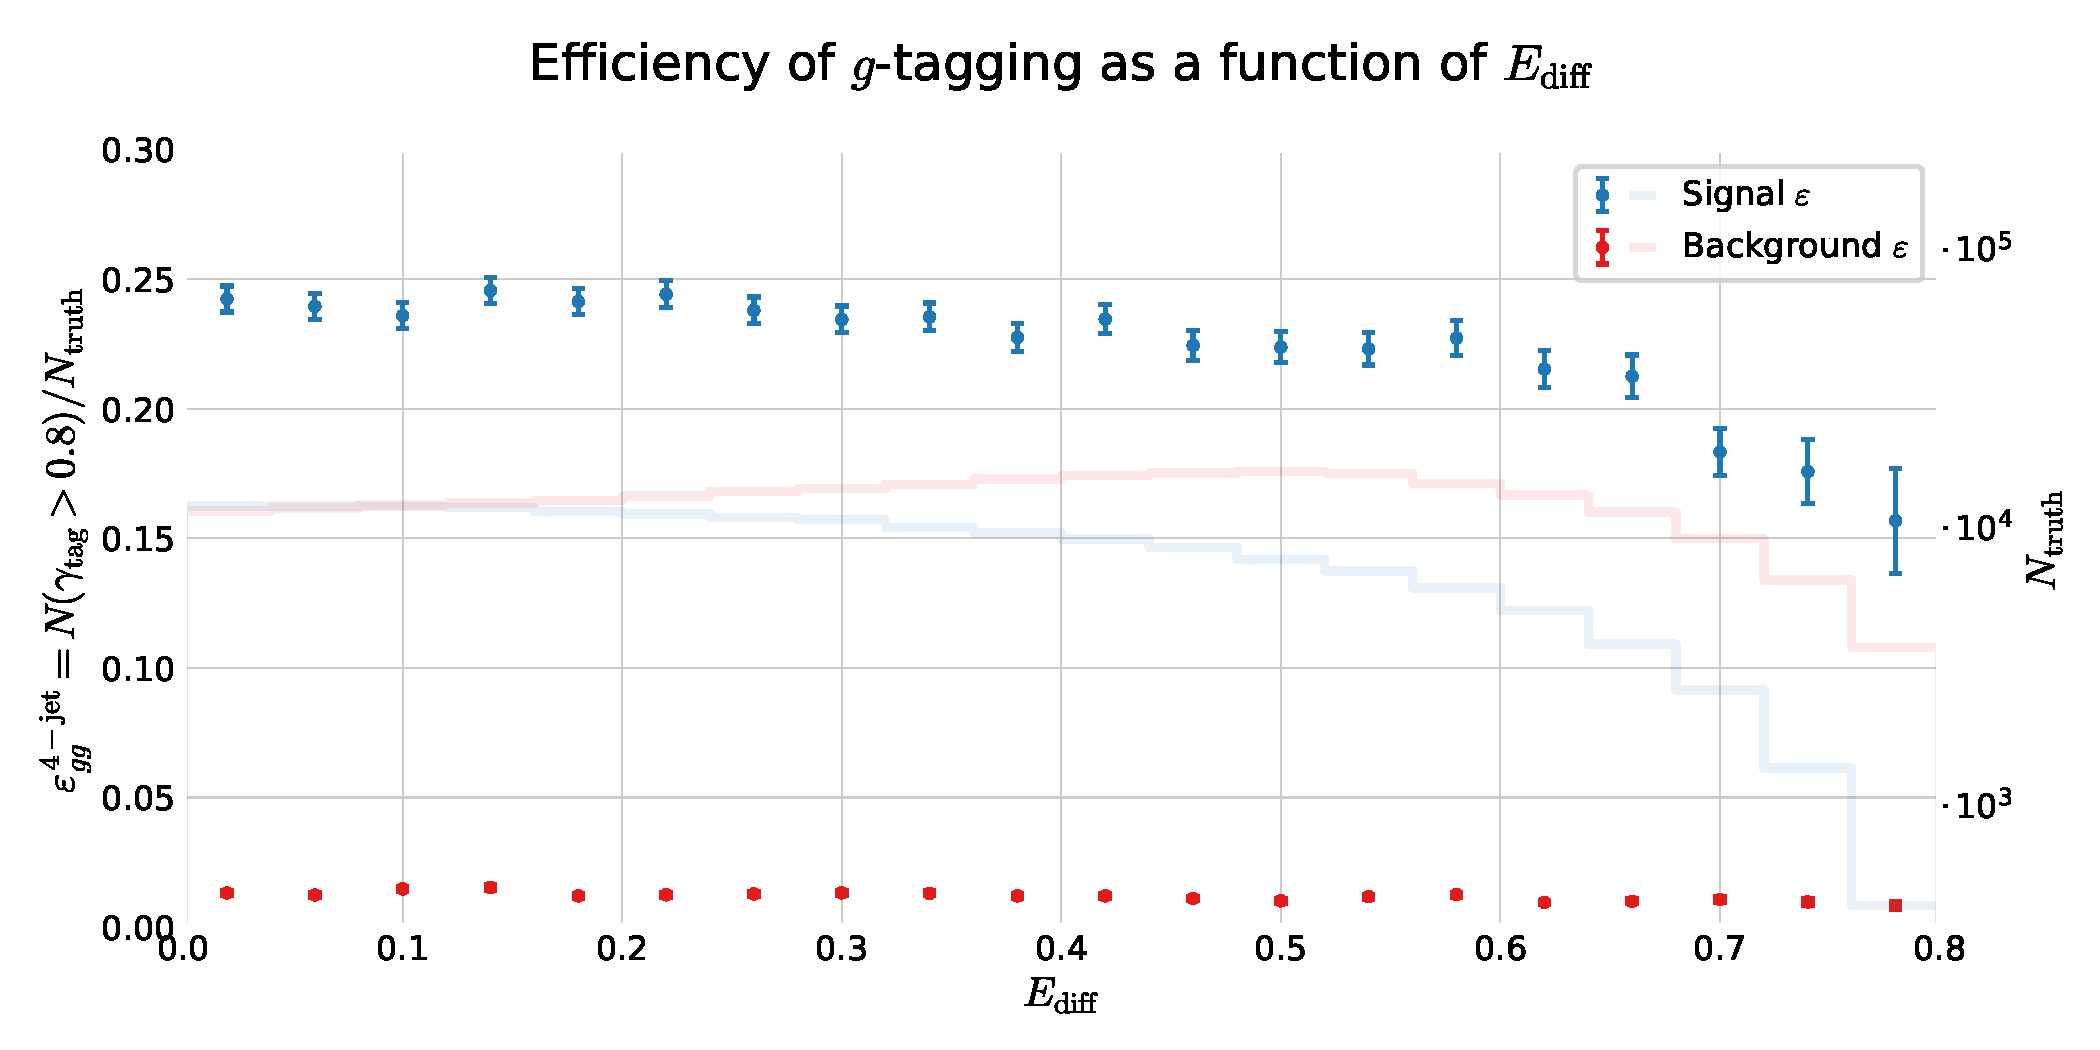
\includegraphics[width=0.95\textwidth, trim=10 10 10 45, clip, page=1]{figures/quarks/efficiency_events-down_sample=1.00-ML_vars=vertex-selection=b-ejet_min=4-n_iter_RS_lgb=99-n_iter_RS_xgb=9-cdot_cut=0.90-version=19-njet=4.pdf}
  \caption[$g$-Tagging Efficiency for 4-Jet Events in MC as a Function of $E_\mathrm{diff}$]
          {Efficiency of the $g$-tagging algorithm for 4-jet events as a function of normalized gluon-gluon jet energy difference (asymmetry) $E_\mathrm{diff}$  in MC. The efficiency is measured as the number of events with a $g$-tag higher than 0.8 ($\gamma > 0.8$) out of the total number. The efficiency is plotted for \textcolor{blue}{signal events} according to MC Truth in blue and \textcolor{red}{background events} according to MC Truth in red.
          } 
  \label{fig:q:effiency_gtag_E_diff}
\end{figure}
\begin{figure}
  \centerfloat
  \includegraphics[width=0.95\textwidth, trim=10 10 10 45, clip, page=2]{figures/quarks/efficiency_events-down_sample=1.00-ML_vars=vertex-selection=b-ejet_min=4-n_iter_RS_lgb=99-n_iter_RS_xgb=9-cdot_cut=0.90-version=19-njet=4.pdf}
  \caption[$g$-Tagging Efficiency for 4-Jet Events in MC as a Function of $E_{\mathrm{rel}_\mathrm{min}}$]
          {Efficiency of the $g$-tagging algorithm for 4-jet events as a function of $E_{\mathrm{rel}_\mathrm{min}}$ in MC. The efficiency is measured as the number of events with a $g$-tag higher than 0.8 ($\gamma > 0.8$) out of the total number. The efficiency is plotted for \textcolor{blue}{signal events} according to MC Truth in blue and \textcolor{red}{background events} according to MC Truth in red.
          } 
  \label{fig:q:effiency_gtag_E_rel_min}
\end{figure}
\begin{figure}
  \centerfloat
  \includegraphics[width=0.95\textwidth, trim=10 10 10 45, clip, page=3]{figures/quarks/efficiency_events-down_sample=1.00-ML_vars=vertex-selection=b-ejet_min=4-n_iter_RS_lgb=99-n_iter_RS_xgb=9-cdot_cut=0.90-version=19-njet=4.pdf}
  \caption[$g$-Tagging Efficiency for 4-Jet Events in MC as a Function of $E_\mathrm{rel}$]
          {Efficiency of the $g$-tagging algorithm for 4-jet events as a function of $E_\mathrm{rel}$  in MC. The efficiency is measured as the number of events with a $g$-tag higher than 0.8 ($\gamma > 0.8$) out of the total number. The efficiency is plotted for \textcolor{blue}{signal events} according to MC Truth in blue and \textcolor{red}{background events} according to MC Truth in red.
          } 
  \label{fig:q:effiency_gtag_E_rel}
\end{figure}
\begin{figure}
  \centerfloat
  \includegraphics[width=0.95\textwidth, trim=10 10 10 45, clip, page=4]{figures/quarks/efficiency_events-down_sample=1.00-ML_vars=vertex-selection=b-ejet_min=4-n_iter_RS_lgb=99-n_iter_RS_xgb=9-cdot_cut=0.90-version=19-njet=4.pdf}
  \caption[$g$-Tagging Efficiency for 4-Jet Events in MC as a Function of $\Delta_\theta$]
          {Efficiency of the $g$-tagging algorithm for 4-jet events as a function of $\Delta_\theta$  in MC. The efficiency is measured as the number of events with a $g$-tag higher than 0.8 ($\gamma > 0.8$) out of the total number. The efficiency is plotted for \textcolor{blue}{signal events} according to MC Truth in blue and \textcolor{red}{background events} according to MC Truth in red.
          } 
  \label{fig:q:effiency_gtag_delta_theta}
\end{figure}
\begin{figure}
  \centerfloat
  \includegraphics[width=0.95\textwidth, trim=10 10 10 45, clip, page=5]{figures/quarks/efficiency_events-down_sample=1.00-ML_vars=vertex-selection=b-ejet_min=4-n_iter_RS_lgb=99-n_iter_RS_xgb=9-cdot_cut=0.90-version=19-njet=4.pdf}
  \caption[$g$-Tagging Efficiency for 4-Jet Events in MC as a Function of $m_{gg}$]
          {Efficiency of the $g$-tagging algorithm for 4-jet events as a function of $m_{gg}$  in MC. The efficiency is measured as the number of events with a $g$-tag higher than 0.8 ($\gamma > 0.8$) out of the total number. The efficiency is plotted for \textcolor{blue}{signal events} according to MC Truth in blue and \textcolor{red}{background events} according to MC Truth in red.
          } 
  \label{fig:q:effiency_gtag_m_gg}
\end{figure}
\begin{figure}
  \centerfloat
  \includegraphics[width=0.95\textwidth, trim=10 10 10 45, clip, page=6]{figures/quarks/efficiency_events-down_sample=1.00-ML_vars=vertex-selection=b-ejet_min=4-n_iter_RS_lgb=99-n_iter_RS_xgb=9-cdot_cut=0.90-version=19-njet=4.pdf}
  \caption[$g$-Tagging Efficiency for 4-Jet Events in MC as a Function of $\phi_\mathrm{\parallel}$]
          {Efficiency of the $g$-tagging algorithm for 4-jet events as a function of $\phi_\mathrm{\parallel}$  in MC. The efficiency is measured as the number of events with a $g$-tag higher than 0.8 ($\gamma > 0.8$) out of the total number. The efficiency is plotted for \textcolor{blue}{signal events} according to MC Truth in blue and \textcolor{red}{background events} according to MC Truth in red.
          } 
  \label{fig:q:effiency_gtag_phi_planes}
\end{figure}
\begin{figure}
  \centerfloat
  \includegraphics[width=0.95\textwidth, trim=10 10 10 45, clip, page=7]{figures/quarks/efficiency_events-down_sample=1.00-ML_vars=vertex-selection=b-ejet_min=4-n_iter_RS_lgb=99-n_iter_RS_xgb=9-cdot_cut=0.90-version=19-njet=4.pdf}
  \caption[$g$-Tagging Efficiency for 4-Jet Events in MC as a Function of $\ln \left( k_t^2 / m_\mathrm{vis}^2 \right)$]
          {Efficiency of the $g$-tagging algorithm for 4-jet events as a function of $\ln \left( k_t^2 / m_\mathrm{vis}^2 \right)$  in MC. The efficiency is measured as the number of events with a $g$-tag higher than 0.8 ($\gamma > 0.8$) out of the total number. The efficiency is plotted for \textcolor{blue}{signal events} according to MC Truth in blue and \textcolor{red}{background events} according to MC Truth in red.
          } 
  \label{fig:q:effiency_gtag_ln_kt_m_vis}
\end{figure}
\begin{figure}
  \centerfloat
  \includegraphics[width=0.95\textwidth, trim=10 10 10 45, clip, page=8]{figures/quarks/efficiency_events-down_sample=1.00-ML_vars=vertex-selection=b-ejet_min=4-n_iter_RS_lgb=99-n_iter_RS_xgb=9-cdot_cut=0.90-version=19-njet=4.pdf}
  \caption[$g$-Tagging Efficiency for 4-Jet Events in MC as a Function of $p^2_{\perp,\mathrm{A}}$]
          {Efficiency of the $g$-tagging algorithm for 4-jet events as a function of $p^2_{\perp,\mathrm{A}}$  in MC. The efficiency is measured as the number of events with a $g$-tag higher than 0.8 ($\gamma > 0.8$) out of the total number. The efficiency is plotted for \textcolor{blue}{signal events} according to MC Truth in blue and \textcolor{red}{background events} according to MC Truth in red.
          } 
  \label{fig:q:effiency_gtag_pt_antenna}
\end{figure}
\begin{figure}
  \centerfloat
  \includegraphics[width=0.95\textwidth, trim=10 10 10 45, clip, page=9]{figures/quarks/efficiency_events-down_sample=1.00-ML_vars=vertex-selection=b-ejet_min=4-n_iter_RS_lgb=99-n_iter_RS_xgb=9-cdot_cut=0.90-version=19-njet=4.pdf}
  \caption[$g$-Tagging Efficiency for 4-Jet Events in MC as a Function of $R_{gg}^\mathrm{k_t}$]
          {Efficiency of the $g$-tagging algorithm for 4-jet events as a function of $R_{gg}^{k_t}$  in MC. The efficiency is measured as the number of events with a $g$-tag higher than 0.8 ($\gamma > 0.8$) out of the total number. The efficiency is plotted for \textcolor{blue}{signal events} according to MC Truth in blue and \textcolor{red}{background events} according to MC Truth in red.
          } 
  \label{fig:q:effiency_gtag_R_gg_kt}
\end{figure}
\begin{figure}
  \centerfloat
  \includegraphics[width=0.95\textwidth, trim=10 10 10 45, clip, page=10]{figures/quarks/efficiency_events-down_sample=1.00-ML_vars=vertex-selection=b-ejet_min=4-n_iter_RS_lgb=99-n_iter_RS_xgb=9-cdot_cut=0.90-version=19-njet=4.pdf}
  \caption[$g$-Tagging Efficiency for 4-Jet Events in MC as a Function of $R_{gg}^\mathrm{CA}$]
          {Efficiency of the $g$-tagging algorithm for 4-jet events as a function of $E$  in MC. The efficiency is measured as the number of events with a $g$-tag higher than 0.8 ($\gamma > 0.8$) out of the total number. The efficiency is plotted for \textcolor{blue}{signal events} according to MC Truth in blue and \textcolor{red}{background events} according to MC Truth in red.
          } 
  \label{fig:q:effiency_gtag_R_gg_CA}
\end{figure}














\FloatBarrier
\newpage

\begin{figure}
  \centerfloat
  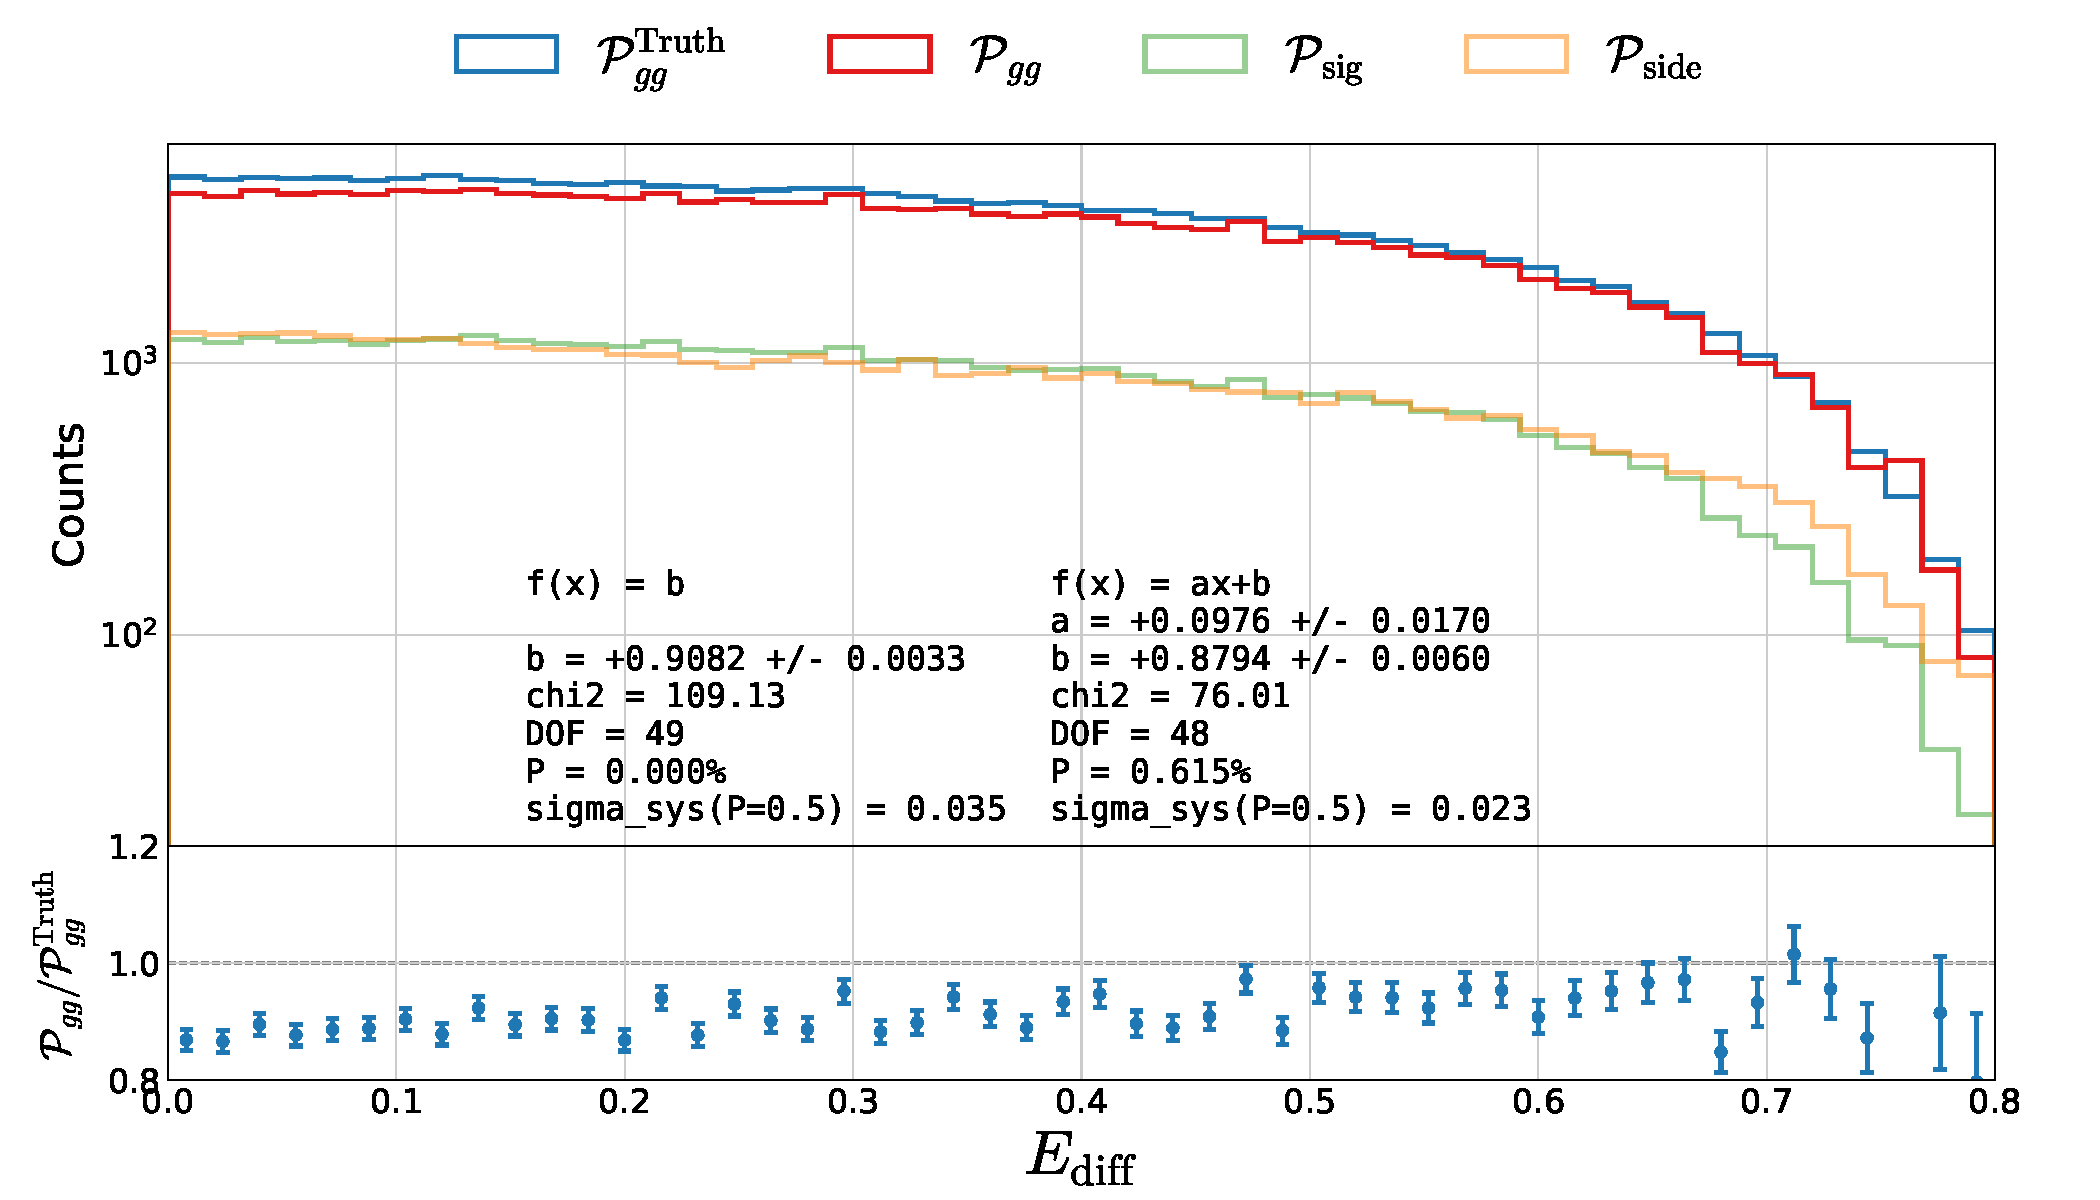
\includegraphics[width=0.99\textwidth, trim=10 0 20 5, clip, page=1]{figures/quarks/gtag-closure_test-down_sample=1.00-ML_vars=vertex-selection=b-ejet_min=4-n_iter_RS_lgb=99-n_iter_RS_xgb=9-cdot_cut=0.90-version=19-njet=4.pdf}
  \caption[Closure Plot Comparing MC Truth and the Efficiency Corrected $g$-Tagging Model in 4-Jet Events for $E_\mathrm{diff}$]
          {Closure plot comparing MC Truth and the efficiency corrected $g$-tagging model in 4-jet events for $E_\mathrm{diff}$. In the top part of the plot \textcolor{blue}{$\mathcal{P}_{gg}^\mathrm{Truth}$} based on MC Truth is shown in blue, the \textcolor{red}{$\mathcal{P}_{gg}$} based on MC but without Truth in red, the distribution in the signal region \textcolor{green}{$\mathcal{P}_{\mathrm{sig}}$} in light green and the distribution in the sideband region \textcolor{orange}{$\mathcal{P}_{\mathrm{side}}$} in light orange. In the bottom part of the plot the ratio between $\mathcal{P}_{gg}$ and $\mathcal{P}_{gg}^\mathrm{Truth}$  is shown. } 
  \label{fig:q:closure_E_diff}
\end{figure}
\begin{figure}
  \centerfloat
  \includegraphics[width=0.99\textwidth, trim=10 0 20 5, clip, page=2]{figures/quarks/gtag-closure_test-down_sample=1.00-ML_vars=vertex-selection=b-ejet_min=4-n_iter_RS_lgb=99-n_iter_RS_xgb=9-cdot_cut=0.90-version=19-njet=4.pdf}
  \caption[Closure Plot Comparing MC Truth and the Efficiency Corrected $g$-Tagging Model in 4-Jet Events for $E_{\mathrm{rel}_\mathrm{min}}$]
          {Closure plot comparing MC Truth and the efficiency corrected $g$-tagging model in 4-jet events for $E_{\mathrm{rel}_\mathrm{min}}$. In the top part of the plot \textcolor{blue}{$\mathcal{P}_{gg}^\mathrm{Truth}$} based on MC Truth is shown in blue, the \textcolor{red}{$\mathcal{P}_{gg}$} based on MC but without Truth in red, the distribution in the signal region \textcolor{green}{$\mathcal{P}_{\mathrm{sig}}$} in light green and the distribution in the sideband region \textcolor{orange}{$\mathcal{P}_{\mathrm{side}}$} in light orange. In the bottom part of the plot the ratio between $\mathcal{P}_{gg}$ and $\mathcal{P}_{gg}^\mathrm{Truth}$  is shown. } 
  \label{fig:q:closure_E_rel_min}
\end{figure}
\begin{figure}
  \centerfloat
  \includegraphics[width=0.99\textwidth, trim=10 0 20 5, clip, page=3]{figures/quarks/gtag-closure_test-down_sample=1.00-ML_vars=vertex-selection=b-ejet_min=4-n_iter_RS_lgb=99-n_iter_RS_xgb=9-cdot_cut=0.90-version=19-njet=4.pdf}
  \caption[Closure Plot Comparing MC Truth and the Efficiency Corrected $g$-Tagging Model in 4-Jet Events for $E_\mathrm{rel}$]
          {Closure plot comparing MC Truth and the efficiency corrected $g$-tagging model in 4-jet events for $E_\mathrm{rel}$. In the top part of the plot \textcolor{blue}{$\mathcal{P}_{gg}^\mathrm{Truth}$} based on MC Truth is shown in blue, the \textcolor{red}{$\mathcal{P}_{gg}$} based on MC but without Truth in red, the distribution in the signal region \textcolor{green}{$\mathcal{P}_{\mathrm{sig}}$} in light green and the distribution in the sideband region \textcolor{orange}{$\mathcal{P}_{\mathrm{side}}$} in light orange. In the bottom part of the plot the ratio between $\mathcal{P}_{gg}$ and $\mathcal{P}_{gg}^\mathrm{Truth}$  is shown. } 
  \label{fig:q:closure_E_rel}
\end{figure}
\begin{figure}
  \centerfloat
  \includegraphics[width=0.99\textwidth, trim=10 0 20 5, clip, page=4]{figures/quarks/gtag-closure_test-down_sample=1.00-ML_vars=vertex-selection=b-ejet_min=4-n_iter_RS_lgb=99-n_iter_RS_xgb=9-cdot_cut=0.90-version=19-njet=4.pdf}
  \caption[Closure Plot Comparing MC Truth and the Efficiency Corrected $g$-Tagging Model in 4-Jet Events for $\Delta_\theta$]
          {Closure plot comparing MC Truth and the efficiency corrected $g$-tagging model in 4-jet events for $\Delta_\theta$. In the top part of the plot \textcolor{blue}{$\mathcal{P}_{gg}^\mathrm{Truth}$} based on MC Truth is shown in blue, the \textcolor{red}{$\mathcal{P}_{gg}$} based on MC but without Truth in red, the distribution in the signal region \textcolor{green}{$\mathcal{P}_{\mathrm{sig}}$} in light green and the distribution in the sideband region \textcolor{orange}{$\mathcal{P}_{\mathrm{side}}$} in light orange. In the bottom part of the plot the ratio between $\mathcal{P}_{gg}$ and $\mathcal{P}_{gg}^\mathrm{Truth}$  is shown. } 
  \label{fig:q:closure_delta_theta}
\end{figure}
\begin{figure}
  \centerfloat
  \includegraphics[width=0.99\textwidth, trim=10 0 20 5, clip, page=5]{figures/quarks/gtag-closure_test-down_sample=1.00-ML_vars=vertex-selection=b-ejet_min=4-n_iter_RS_lgb=99-n_iter_RS_xgb=9-cdot_cut=0.90-version=19-njet=4.pdf}
  \caption[Closure Plot Comparing MC Truth and the Efficiency Corrected $g$-Tagging Model in 4-Jet Events for $m_{gg}$]
          {Closure plot comparing MC Truth and the efficiency corrected $g$-tagging model in 4-jet events for $m_{gg}$. In the top part of the plot \textcolor{blue}{$\mathcal{P}_{gg}^\mathrm{Truth}$} based on MC Truth is shown in blue, the \textcolor{red}{$\mathcal{P}_{gg}$} based on MC but without Truth in red, the distribution in the signal region \textcolor{green}{$\mathcal{P}_{\mathrm{sig}}$} in light green and the distribution in the sideband region \textcolor{orange}{$\mathcal{P}_{\mathrm{side}}$} in light orange. In the bottom part of the plot the ratio between $\mathcal{P}_{gg}$ and $\mathcal{P}_{gg}^\mathrm{Truth}$  is shown. } 
  \label{fig:q:closure_m_gg}
\end{figure}
\begin{figure}
  \centerfloat
  \includegraphics[width=0.99\textwidth, trim=10 0 20 5, clip, page=6]{figures/quarks/gtag-closure_test-down_sample=1.00-ML_vars=vertex-selection=b-ejet_min=4-n_iter_RS_lgb=99-n_iter_RS_xgb=9-cdot_cut=0.90-version=19-njet=4.pdf}
  \caption[Closure Plot Comparing MC Truth and the Efficiency Corrected $g$-Tagging Model in 4-Jet Events for $\phi_\mathrm{\parallel}$]
          {Closure plot comparing MC Truth and the efficiency corrected $g$-tagging model in 4-jet events for $\phi_\mathrm{\parallel}$. In the top part of the plot \textcolor{blue}{$\mathcal{P}_{gg}^\mathrm{Truth}$} based on MC Truth is shown in blue, the \textcolor{red}{$\mathcal{P}_{gg}$} based on MC but without Truth in red, the distribution in the signal region \textcolor{green}{$\mathcal{P}_{\mathrm{sig}}$} in light green and the distribution in the sideband region \textcolor{orange}{$\mathcal{P}_{\mathrm{side}}$} in light orange. In the bottom part of the plot the ratio between $\mathcal{P}_{gg}$ and $\mathcal{P}_{gg}^\mathrm{Truth}$  is shown. } 
  \label{fig:q:closure_phi_planes}
\end{figure}
\begin{figure}
  \centerfloat
  \includegraphics[width=0.99\textwidth, trim=10 0 20 5, clip, page=7]{figures/quarks/gtag-closure_test-down_sample=1.00-ML_vars=vertex-selection=b-ejet_min=4-n_iter_RS_lgb=99-n_iter_RS_xgb=9-cdot_cut=0.90-version=19-njet=4.pdf}
  \caption[Closure Plot Comparing MC Truth and the Efficiency Corrected $g$-Tagging Model in 4-Jet Events for $\ln \left( k_t^2 / m_\mathrm{vis}^2 \right)$]
          {Closure plot comparing MC Truth and the efficiency corrected $g$-tagging model in 4-jet events for $\ln \left( k_t^2 / m_\mathrm{vis}^2 \right)$. In the top part of the plot \textcolor{blue}{$\mathcal{P}_{gg}^\mathrm{Truth}$} based on MC Truth is shown in blue, the \textcolor{red}{$\mathcal{P}_{gg}$} based on MC but without Truth in red, the distribution in the signal region \textcolor{green}{$\mathcal{P}_{\mathrm{sig}}$} in light green and the distribution in the sideband region \textcolor{orange}{$\mathcal{P}_{\mathrm{side}}$} in light orange. In the bottom part of the plot the ratio between $\mathcal{P}_{gg}$ and $\mathcal{P}_{gg}^\mathrm{Truth}$  is shown. } 
  \label{fig:q:closure_ln_kt_m_vis}
\end{figure}
\begin{figure}
  \centerfloat
  \includegraphics[width=0.99\textwidth, trim=10 0 20 5, clip, page=8]{figures/quarks/gtag-closure_test-down_sample=1.00-ML_vars=vertex-selection=b-ejet_min=4-n_iter_RS_lgb=99-n_iter_RS_xgb=9-cdot_cut=0.90-version=19-njet=4.pdf}
  \caption[Closure Plot Comparing MC Truth and the Efficiency Corrected $g$-Tagging Model in 4-Jet Events for $p^2_{\perp,\mathrm{A}}$]
          {Closure plot comparing MC Truth and the efficiency corrected $g$-tagging model in 4-jet events for $p^2_{\perp,\mathrm{A}}$. In the top part of the plot \textcolor{blue}{$\mathcal{P}_{gg}^\mathrm{Truth}$} based on MC Truth is shown in blue, the \textcolor{red}{$\mathcal{P}_{gg}$} based on MC but without Truth in red, the distribution in the signal region \textcolor{green}{$\mathcal{P}_{\mathrm{sig}}$} in light green and the distribution in the sideband region \textcolor{orange}{$\mathcal{P}_{\mathrm{side}}$} in light orange. In the bottom part of the plot the ratio between $\mathcal{P}_{gg}$ and $\mathcal{P}_{gg}^\mathrm{Truth}$  is shown. } 
  \label{fig:q:closure_variable_pt_antenna}
\end{figure}








\FloatBarrier
\newpage

\begin{figure*}[h!]
  \centerfloat
  \includegraphics[width=0.95\textwidth, trim=0 0 0 0, clip, page=1]{figures/quarks/gtag-R_kt_CA_histograms-down_sample=1.00-ML_vars=vertex-selection=b-ejet_min=4-n_iter_RS_lgb=99-n_iter_RS_xgb=9-cdot_cut=0.90-version=19-njet=4.pdf}
  \caption[Gluon Splitting Distribution Comparison in MC and Data for $R_{gg}^{k_t}$-$R_{gg}^\mathrm{CA}$ Phase Space Area A]
          {Comparison of the gluon splitting distributions in MC and Data for $R_{gg}^{k_t}$-$R_{gg}^\mathrm{CA}$ Phase Space Area A, see Table~\ref{tab:q:gluon_splitting_area_definitions}. The distribution for \textcolor{blue}{MC} (scaled to Data) is shown in blue and for \textcolor{red}{Data} in red. These eight distributions are for the $R_{gg}^{k_t}$-$R_{gg}^\mathrm{CA}$ Phase Space Area A which has \num{5022} events in the MC sample and \num{3111} in the Data sample. } 
  \label{fig:q:R_kt_CA_cut_A}
\end{figure*}

\begin{figure*}[h!]
  \centerfloat
  \includegraphics[width=0.95\textwidth, trim=0 0 0 0, clip, page=2]{figures/quarks/gtag-R_kt_CA_histograms-down_sample=1.00-ML_vars=vertex-selection=b-ejet_min=4-n_iter_RS_lgb=99-n_iter_RS_xgb=9-cdot_cut=0.90-version=19-njet=4.pdf}
  \caption[Gluon Splitting Distribution Comparison in MC and Data for $R_{gg}^{k_t}$-$R_{gg}^\mathrm{CA}$ Phase Space Area B]
          {Comparison of the gluon splitting distributions in MC and Data for $R_{gg}^{k_t}$-$R_{gg}^\mathrm{CA}$ Phase Space Area B, see Table~\ref{tab:q:gluon_splitting_area_definitions}. The distribution for \textcolor{blue}{MC} (scaled to Data) is shown in blue and for \textcolor{red}{Data} in red. These eight distributions are for the $R_{gg}^{k_t}$-$R_{gg}^\mathrm{CA}$ Phase Space Area B which has \num{7382} events in the MC sample and \num{4035} in the Data sample. } 
  \label{fig:q:R_kt_CA_cut_B}
\end{figure*}

\begin{figure*}[h!]
  \centerfloat
  \includegraphics[width=0.95\textwidth, trim=0 0 0 0, clip, page=3]{figures/quarks/gtag-R_kt_CA_histograms-down_sample=1.00-ML_vars=vertex-selection=b-ejet_min=4-n_iter_RS_lgb=99-n_iter_RS_xgb=9-cdot_cut=0.90-version=19-njet=4.pdf}
  \caption[Gluon Splitting Distribution Comparison in MC and Data for $R_{gg}^{k_t}$-$R_{gg}^\mathrm{CA}$ Phase Space Area C]
          {Comparison of the gluon splitting distributions in MC and Data for $R_{gg}^{k_t}$-$R_{gg}^\mathrm{CA}$ Phase Space Area C, see Table~\ref{tab:q:gluon_splitting_area_definitions}. The distribution for \textcolor{blue}{MC} (scaled to Data) is shown in blue and for \textcolor{red}{Data} in red. These eight distributions are for the $R_{gg}^{k_t}$-$R_{gg}^\mathrm{CA}$ Phase Space Area C which has \num{9417} events in the MC sample and \num{5344} in the Data sample. } 
  \label{fig:q:R_kt_CA_cut_C}
\end{figure*}

\begin{figure*}[h!]
  \centerfloat
  \includegraphics[width=0.95\textwidth, trim=0 0 0 0, clip, page=4]{figures/quarks/gtag-R_kt_CA_histograms-down_sample=1.00-ML_vars=vertex-selection=b-ejet_min=4-n_iter_RS_lgb=99-n_iter_RS_xgb=9-cdot_cut=0.90-version=19-njet=4.pdf}
  \caption[Gluon Splitting Distribution Comparison in MC and Data for $R_{gg}^{k_t}$-$R_{gg}^\mathrm{CA}$ Phase Space Area D]
          {Comparison of the gluon splitting distributions in MC and Data for $R_{gg}^{k_t}$-$R_{gg}^\mathrm{CA}$ Phase Space Area D, see Table~\ref{tab:q:gluon_splitting_area_definitions}. The distribution for \textcolor{blue}{MC} (scaled to Data) is shown in blue and for \textcolor{red}{Data} in red. These eight distributions are for the $R_{gg}^{k_t}$-$R_{gg}^\mathrm{CA}$ Phase Space Area D which has \num{26366} events in the MC sample and \num{13780} in the Data sample. } 
  \label{fig:q:R_kt_CA_cut_D}
\end{figure*}